\ExerciseSection

\begin{enumerate}
\def\labelenumi{\arabic{enumi})}
\tightlist
\item
  设 \(f(z) = z^n + a_1z^{n-1} + \cdots + a_{n-1}z + a_n\) 是一个 \(n\) 次复系数多项式，并令 \(f(z) = \prod_{i=1}^{n}(z - z_i)\) 。令 \(r_0 = \sup_i |z_i|\) 。
\end{enumerate}

\begin{enumerate}
\def\labelenumi{\alph{enumi})}
\tightlist
\item
  证明：若实数 \(r > 0\) 满足
\end{enumerate}

\[
r ^ {n} \leqslant | a _ {1} | r ^ {n - 1} + | a _ {2} | r ^ {n - 2} + \dots + | a _ {n - 1} | r + | a _ {n} |,
\]

则 \(r_0 \leqslant r\) ，并由此推出

\[
r _ {0} \leqslant \sup \left(\mathrm{I}, \sum_ {k = 1} ^ {n} | a _ {k} |\right).
\]

\begin{enumerate}
\def\labelenumi{\alph{enumi})}
\setcounter{enumi}{1}
\item
  设 \((\lambda_i)_{1 \leqslant i \leqslant n}\) 是由 \(n\) 个 \(>0\) 的实数组成的有限序列，且满足 \(\sum_{i=1}^{n} \lambda_i^{-1} = 1\) 。证明 \(r_0 \leqslant \sup_k (\lambda_k |a_k|)^{1/k}\) {[}利用 \(a\){]} 。
\item
  由 \(a\) ) 推出：若诸系数 \(a_i\) 都不为零，则
\end{enumerate}

\[
r _ {0} \leqslant \sup \left(2 | a _ {1} |, 2 \left| \frac {a _ {2}}{a _ {1}} \right|, \dots , 2 \left| \frac {a _ {n - 1}}{a _ {n - 2}} \right|, \left| \frac {a _ {n}}{a _ {n - 1}} \right|\right).
\]

\begin{enumerate}
\def\labelenumi{\alph{enumi})}
\setcounter{enumi}{3}
\tightlist
\item
  由 a) 推出
\end{enumerate}

\[
r _ {0} \leqslant | a _ {1} - 1 | + | a _ {2} - a _ {1} | + \dots + | a _ {n - 1} - a _ {n} | + | a _ {n} |
\]

{[}考虑多项式 \((z - 1)f(z)]\) 。由此证明：若诸 \(a_i\) 都是实数且 \(>0\) ，则

\[
r _ {0} \leqslant \sup \left(a _ {1}, \frac {a _ {2}}{a _ {1}}, \dots , \frac {a _ {n - 1}}{a _ {n - 2}}, \frac {a _ {n}}{a _ {n - 1}}\right).
\]

\begin{enumerate}
\def\labelenumi{\arabic{enumi})}
\setcounter{enumi}{1}
\tightlist
\item
  代数数是在有理数域 \(\mathbf{Q}\) 上为代数的复数。证明由全体实代数数组成的序域 \(\mathbf{B}\) 是一个极大序域，但它对于由 \(\mathbf{R}\) 诱导的拓扑并不完备{[}这一拓扑与 \(\mathcal{C}_0(\mathbf{B})\) 相同；参看第四章，§ 3，习题 2 b){]}。
\end{enumerate}

¶ 3) a) 设 K 是一个极大序域，赋有拓扑 \(\mathfrak{G}_{0}(\mathbf{K})\) ，该拓扑与其域结构相容（第四章，§ 3，习题 2）。设

\[
f (\mathbf {X}) = a _ {0} \mathbf {X} ^ {n} + a _ {1} \mathbf {X} ^ {n - 1} + \dots + a _ {n}
\]

是 K{[}X{]} 中在 K 内有一个单根 \(\alpha\) 的多项式。证明：对 K 中每个元素 \(\varepsilon > 0\) ，存在 K 中的 \(\eta > 0\) ，使得每个多项式 \(g(\mathbf{X}) = b_{0}\mathbf{X}^{n} + b_{1}\mathbf{X}^{n-1} + \cdots + b_{n}\) ，只要对一切 i 有 \(|a_{i} - b_{i}| \leqslant \eta\) ，就恰有一个单根 \(\beta\) 满足 \(|\beta - \alpha| \leqslant \varepsilon\) 。（把 f 与 g 按 X - \(\alpha\) 的幂展开。）给出 \(\eta\) 关于 \(a_{i}, \alpha\) 与 \(\varepsilon\) 的一个上界。

\begin{enumerate}
\def\labelenumi{\alph{enumi})}
\setcounter{enumi}{1}
\item
  推出：若 K 是极大序域，则它的完备化 \(\hat{K}\) （关于 \(\mathcal{G}_{0}(K)\) ；这是一个带有自然序结构的域：第四章，§ 4，习题 2）是极大序域。
\item
  设 \(K_{0}\) 是一个序域，并设 \(S = K_{0}((X))\) 是 \(K_{0}\) 上一个未定元的形式幂级数域；把 S 中 \(\geqslant 0\) 的元素取为 o 以及最低次项系数 \textgreater0 的形式幂级数，以此给 S 一个线性序。证明赋有拓扑 \(\mathcal{G}_{0}(S)\) 的 S 是完备的，但 S 不是极大序域（证明多项式 \(Y^{p} - X\) 在 S{[}Y{]} 中对每个整数 p \textgreater{} 1 都不可约）。
\end{enumerate}

\(d\) ) 在 \(c\) ) 的例子中取 \(\mathbf{K}_0 = \mathbb{R}\) 。设 \(\mathbf{K}\) 是 \(\mathbf{S}\) 的一个极大序代数扩张；证明 \(\mathbf{K}\) 在拓扑 \(\mathfrak{C}_0(\mathbf{K})\) 下不完备。（把 \(\mathbf{S}\) 嵌入以良序指数的形式幂级数所成的域 \(\mathbf{E}\) ，其序按与 \(\mathbf{S}\) 相同的方式给定，再把 \(\mathbf{K}\) 嵌入 \(\Omega\) —— \(\mathbf{E}\) 的一个极大序扩张 —— 。注意 \(\mathbf{E}\) 是完备的，并给出 \(\mathbf{K}\) 中一个柯西序列的例子，它收敛于一个元素 \(f \in \mathbf{E}\) ，该元素在 \(\mathbf{S}\) 上不是代数的；如此选取 \(f\) ，使得存在无穷多个 \(\mathbf{E}\) 到 \(\Omega\) 的一个代数闭包中的 S-同构，并且 \(f\) 在这些同构下的像两两不同。{]}

\begin{enumerate}
\def\labelenumi{\arabic{enumi})}
\setcounter{enumi}{3}
\tightlist
\item
  证明：\(f\) 若是拓扑域 \(\mathbf{C}\) 到 \(\mathbf{C}\) 的一个子域上的连续同态（必然是单射），则它或是恒等自同构，或是自同构 \(z \to \overline{z}\) 。 {[}注意必须 \(f(x) = x\) 对一切 \(x \in \mathbf{Q}\) 成立，并由此推出 \(f(x) = x\) 对一切 \(x \in \mathbf{R}\) 成立。{]}证明存在无穷多个 \(\mathbf{C}\) 到 \(\mathbf{C}\) 的异于 \(\mathbf{C}\) 本身的子域上的不连续同构。
\end{enumerate}

¶ 5) a) 设 K 是四元数体 H 的一个非交换子体；证明 K 的中心 Z 是 H 的中心 R 的一个子域。（注意 K 的每个元素与由 Z ∪ R 生成的域 L 的每个元素交换；若 Z ⊕ R ，则域 L 将是 H 的一个极大子域，而 K 将包含于 L 中，与假设矛盾。）

\begin{enumerate}
\def\labelenumi{\alph{enumi})}
\setcounter{enumi}{1}
\tightlist
\item
  推出：\(f\) （不必连续）若是 \(\mathbf{H}\) 到 \(\mathbf{H}\) 的一个子体上的同构，则它是形如 \(x \to axa^{-1}\) 的一个 \(\mathbf{H}\) 的内自同构。 {[}\(f\) 在 \(\mathbf{R}\) 上的限制是 \(\mathbf{R}\) 到 \(\dot{\mathbf{R}}\) 的一个子域上的同构，这由 \(a\) ) 得出；利用第四章 § 3 的习题 3。{]}
\end{enumerate}

\ExerciseSection

\begin{enumerate}
\def\labelenumi{\arabic{enumi})}
\item
  设 \(a\) 是一个非零复数，\(n\) 是一个 \(>0\) 的整数。对每个实数 \(r > 0\) （满足 \(r^n \leqslant |a|\) ），证明存在 \(z \in \mathbf{C}\) 使得 \(|z| = r\) 且 \(|a + z^n| = |a| - r^n\) 。由此推出：若 \(f\) 是次数 \(>0\) 的复系数多项式，则不等式 \(|f(z_0)| \leqslant |f(z)|\) 不可能对一个邻域中的所有点 \(z\) 成立，该邻域属于某点 \(z_0\) ，只要 \(f(z_0) \neq 0\) 。
\item
  证明：若 \(f\) 是任一复系数多项式且不恒等于零，则存在实数 \(r > 0\) 使得
\end{enumerate}

\[
\left| f (z) \right| > \left| f (\mathbf {o}) \right|
\]

对一切满足 \(|z| \geqslant r\) 的 z 成立。于是，借助习题 1 与魏尔斯特拉斯定理（第四章，§ 6，第 1 号，定理 1），给出 \(\mathbf{C}\) 是代数闭域这一事实的另一个证明（考察函数 \(f\) 在由点 \(z\) （满足 \(|z| \leqslant r\) ）组成的紧集上的情况）。

\begin{enumerate}
\def\labelenumi{\arabic{enumi})}
\setcounter{enumi}{2}
\item
  不利用定理 1 证明：映射 \(z \to z / \overline{z}\) 是拓扑群 \(\mathbf{C}^*\) 到拓扑群 \(\mathbf{U}\) 上的一个严格态射。由此推出：映射 \(t \to (\mathrm{i} + it) / (\mathrm{i} - it) \left[ (\mathrm{i} + it) / (\mathrm{i} - it) = -\mathrm{i} \right.\) （若 \(t = \infty\) ）是拓扑群 \(\tilde{\mathbf{R}}\) （第 6 号）到拓扑群 \(\mathbf{U}\) 上的一个同构，从而给出定理 1 的另一个证明。
\item
  设 K 是 R 的最小毕达哥拉斯子域，并设 \(\mathrm{K}^{\prime}=\mathrm{K}(i)\) 。设 G 是 \(K^{\prime}\) 中绝对值为 1 的元素所成的乘法群（U 的一个子群）。证明 G 不同构于 K 中数 mod 1 的加法群。（注意在后一群中存在任意素数阶 p 的元素；另一方面，若 p 是使 p-1 不是 2 的方幂的素数，则注意 \(K^{\prime}\) 的每个元素在 Q 上的次数都是 2 的方幂，由此证明 G 中除 1 外不含 p 次单位根。）
\end{enumerate}

\ExerciseSection

¶ 1) 对复数的每个有限序列 \(s = (z_k)_{k \in \mathbf{I}}\) ，令

\[
\sum_ {k \in \mathbf {I}} | z _ {k} | = \rho_ {s} \cdot \sup _ {\mathbf {J} \subset \mathbf {I}} \left| \sum_ {k \in \mathbf {J}} z _ {k} \right|
\]

（参看第七章，§ 3，第 1 号，命题 2）。

\begin{enumerate}
\def\labelenumi{\alph{enumi})}
\tightlist
\item
  * 若 \(z_{k} = r_{k} (\cos \varphi_{k} + i \sin \varphi_{k})\) ，其中 \(r_{k} = |z_{k}|\) ，而 \(\varphi_{k}\) 是 \(z_{k}\) 的辐角的主弧度测度，令
\end{enumerate}

\[
f (\varphi) = \sum_ {k \in \mathbf {I}} r _ {k} (\cos (\varphi - \varphi_ {k})) ^ {+}
\]

对每个 \(\varphi \in [0, 2\pi[\) 成立。证明 \(f(\varphi)\) 在区间 \([0, 2\pi[\) 中的上确界等于 \(\sup_{J \subset I} \left| \sum_{k \in J} z_k \right|\) 。考察积分 \(\int_0^{2\pi}f(\varphi)d\varphi\) ，推出：对一切有限序列 \(s\) 有 \(\rho_{s}\leqslant \pi\) ，且不存在有限序列 \((z_k) = s\) 使得 \(\rho_{s} = \pi\)

\begin{enumerate}
\def\labelenumi{\alph{enumi})}
\setcounter{enumi}{1}
\tightlist
\item
  证明：对每个 \(\varepsilon > 0\) ，存在有限序列 \((z_k) = s\) 使得 \(\rho_s > \pi - \varepsilon\) （取 \(z_k\) 为一个次数足够高的二项方程的根）。*
\end{enumerate}

\begin{enumerate}
\def\labelenumi{\arabic{enumi})}
\setcounter{enumi}{1}
\tightlist
\item
  设 \((z_{n})\) 是复数的无穷序列 \(z_{n} = x_{n} + iy_{n}\) ，使得 \(x_{n} \geqslant 0\) 对一切 \(n\) 成立。证明：若以 \(z_{n}\) 与 \(z_{n}^{2}\) 为通项的级数都收敛，则以 \(z_{n}^{2}\) 为通项的级数绝对收敛。给出一个例子，说明当把条件 \(x_{n} \geqslant 0\) （它也可写成 \(-\pi / 2 \leqslant \operatorname{Am}(z_{n}) \leqslant \pi / 2\) ）换成
\end{enumerate}

\[
- (\mathrm{I} - \varepsilon) \frac {\pi}{2} \leqslant \operatorname{Am} (z _ {n}) \leqslant (\mathrm{I} + \varepsilon) \frac {\pi}{2}
\]

时，无论实数 \(\varepsilon > 0\) 多么小，该结果都可能不成立。（这里 Am \((z)\) 表示 \(z_{n}\) 的辐角的属于区间 \([- \pi, +\pi]\) 的那个弧度测度。）

\begin{enumerate}
\def\labelenumi{\arabic{enumi})}
\setcounter{enumi}{2}
\item
  设 \((z_{t})_{t\in I}\) 是一族复数，使得 \(\prod_{t\in I}|z_t| = +\infty\) （相应地 \(\prod_{t\in I}|z_t| = 0\) ）。证明族 \((z_{t})\) 在空间 \(\tilde{\mathbf{C}}\) （ \(\S 4\) ，第 3 号）中可乘，且其乘积为 \(\infty\) （相应地为 0）。
\item
  证明以 \(1 + i/n\) 为通项因子的无穷乘积不收敛，但其因子的绝对值之乘积绝对收敛。
\item
  设 \((z_{n})\) 是非零复数的无穷序列，使得 \(\lim_{n\to \infty}z_n = 1\) 。证明：若 \(\sigma\) 是 \(\mathbf{N}\) 的一个置换，使得以 \(z_{\sigma (n)}\) 为通项因子的无穷乘积收敛，则诸乘积
\end{enumerate}

\[
\underset {n = 0} {\overset {\infty} {\mathbf {P}}} z _ {\sigma (n)}
\]

所成的集，当取遍所有这些置换时，可以是：(i) 单个点；或 (ii) 整个群 \(\mathbf{C}^*\) ；或 (iii) 以 \(\mathbf{o}\) 为端点的一条开射线；或 (iv) 以 \(\mathbf{o}\) 为圆心的一个圆周；或 (v) 一条“对数螺线”，即 \(\mathbf{R}\) 在映射 \(t \to a^{t - t_0} (\cos t + i \sin t)\) 下的像，其中 \(a\) 是 \(>0\) 且 \(\neq 1\) 的实数。（利用乘法群 \(\mathbf{C}^*\) 同构于加法群 \(\mathbf{R} \times \mathbf{T}\) 这一事实，按第七章 § 3 习题 2 的方式论证。）

\ExerciseSection

\begin{enumerate}
\def\labelenumi{\arabic{enumi})}
\item
  设 \(f\) 是 \(n\) 个复变量的多项式，系数为复数且不恒等于零。证明 \(\mathbf{C}^n\) 中集 \(S\) 的余集是连通的，这里 S 是由点 \(z = (z_i)\) （满足 \(f(z_1, z_2, \ldots, z_n) = 0\) ；即方程为 \(f = 0\) 的“代数簇”）所组成的集。（若 \(a, b\) 是 \(\mathbb{C}S\) 的两个不同点，考察 \(S\) 与过 \(a\) 和 \(b\) 的复直线的交。）
\item
  设 K 是一个非离散的豪斯多夫拓扑除环（或域）。
\end{enumerate}

\begin{enumerate}
\def\labelenumi{\alph{enumi})}
\tightlist
\item
  设 E 是 K 上的一个 n 维左向量空间。若 \((a_{i})_{1\leqslant i\leqslant n}\) 是 E 的一个基，并且借助双射线性映射把 \(K^{n}\) 的拓扑（诸因子拓扑的乘积）转移到 E 上
\end{enumerate}

\[
(x _ {i}) \rightarrow \sum_ {i = 1} ^ {n} x _ {i} a _ {i},
\]

则这样在 E 上定义的拓扑与所选取的基 \((a_{i})\) 无关，它与 E 的加法群结构相容，并且使映射 \((t, x) \to tx\) （它把 \(K \times E\) 映入 E）连续。若 F 是 E 的一个向量子空间，则 E 的拓扑在 F 上诱导的拓扑与从 F 的任意一个基出发按上述方式在 F 上定义的拓扑相同；F 在 E 中是闭的，并且除非 F = E，CF 在 E 中稠密。

\begin{enumerate}
\def\labelenumi{\alph{enumi})}
\setcounter{enumi}{1}
\tightlist
\item
  把第六章 § 1 的命题 4、5 与 6 推广到除环 K。（为证明当 K 非交换时映射 \(X \to X^{-1}\) 在 K 上每个 n 阶非奇异方阵的邻域内连续，对 n 用归纳法：考察 n 阶单位矩阵 \(I_{n}\) 的一个邻域，注意每个充分接近 \(I_{n}\) 的矩阵 X 都可表成形式
\end{enumerate}

\[
\left( \begin{array}{c c c c} \mathrm{I} & \mathrm{O} & \ldots & \mathrm{O} \\ \lambda_ {2} & & & \\ \vdots & & I _ {n - 1} & \\ \lambda_ {n} & & & \end{array} \right) \left( \begin{array}{c c c c} \mu_ {1} & \mu_ {2} & \ldots & \mu_ {n} \\ \mathrm{o} & & & \\ \vdots & & Y & \\ \mathrm{o} & & & \end{array} \right),
\]

其中 \(I_{n-1}\) 是 n−i 阶单位矩阵，而 Y 是 n−i 阶非奇异矩阵。）

\begin{enumerate}
\def\labelenumi{\alph{enumi})}
\setcounter{enumi}{2}
\item
  若 K 交换且 E 是 K 上秩为 n 的一个代数，则 E 的拓扑与其环结构相容。此外，若 E 有单位元，则 E 的单位群 G 在 E 中是开的且稠密，并且 E 的拓扑在 G 上诱导的拓扑与 G 的群结构相容。（若 e 是 E 的单位元且 x 是 E 的一个单位，则方程 xy = e 与 yx = e 各有且仅有一个解 y；对这两个方程中的每一个，考察给出 y 关于 E 的某个基的分量的等价 n 元线性方程组。）
\item
  若 K 是不完备的域而 E 是 K 上秩为 n 的代数，且 K 的完备化 \(\hat{K}\) 是一个域，则代数 E 的完备化 \(\hat{E}\) 就是把 E 的算子环扩张到 \(\hat{K}\) 而得到的那个代数。由此构造一些完备化不是除环的拓扑除环的例子。
\end{enumerate}

\begin{enumerate}
\def\labelenumi{\arabic{enumi})}
\setcounter{enumi}{2}
\item
  利用第一章 § 3 第 6 号的命题 10，证明实射影空间 \(\mathbf{P}_{n}(\mathbf{R})\) 同胚于 \(\mathbf{P}_{n}(\mathbf{C})\) 的由至少具有一组实齐次坐标的那些点组成的子空间。\([\mathbf{R}_{n+1}^{*}\) 看作嵌入在 \(\mathbf{C}_{n+1}^{*}\) 中，设 A 是 \(\mathbf{R}_{n+1}^{*}\) 中的一个闭集，关于 \(\Delta_{n}(\mathbf{R})\) 是饱和的；设 B 是所有点 \(\zeta x\) 所成的集，其中 \(x \in A\) 且 \(\zeta \in U\) ；证明 \(\overline{\mathbf{B}}\) 关于 \(\Delta_{n}(\mathbf{C})\) 是饱和的，且 A 是 \(\overline{\mathbf{B}}\) 在 \(\mathbf{R}_{n+1}^{*}\) 上的迹。{]}
\item
  在 \(\mathbf{P}_{n}(\mathbf{C})\) 中，设 \(H_{n}\) 是由方程
\end{enumerate}

\[
x _ {0} ^ {2} + x _ {1} ^ {2} + \dots + x _ {n} ^ {2} = 0.
\]

所定义的“二次超曲面”。证明 \(H_{n}\) 的每个点都有一个同胚于 \(C^{n-1}\) 的开邻域，\(H_{n}\) 是连通的，并且 \(H_{n}\) 与任一复射影超平面的余集之交是连通的（为证最后这一断言，化归到 \(n = 2\) 的情形）。

证明 \(H_{2}\) 同胚于 \(S_{2}\) ，而 \(H_{3}\) 同胚于 \(S_{2} \times S_{2}\) （利用二次曲面借助于其直母线的参数表示）。

\begin{enumerate}
\def\labelenumi{\arabic{enumi})}
\setcounter{enumi}{4}
\tightlist
\item
  把球面 \(\mathbf{S}_5\) 看作 \(\mathbf{C}^3\) 的子空间，考察 \(\mathbf{S}_5\) 到 \(\mathbf{R}^7\) 中的映射，它把每个点 \(x = (x_1, x_2, x_3)\) （属于 \(\mathbf{S}_5\) ， \(x_1, x_2, x_3\) 为复数）映到点 \(y = (y_i)_{1 \leqslant i \leqslant 7}\) （属于 \(\mathbf{R}^7\) ），其中
\end{enumerate}

\[
\begin{array}{c} y _ {1} = | x _ {1} | ^ {2} - | x _ {2} | ^ {2}, \quad y _ {2} = \mathcal {R} (x _ {1} \overline {{x}} _ {2}), \quad y _ {3} = \mathcal {I} (x _ {1} \overline {{x}} _ {2}), \quad y _ {4} = \mathcal {R} (x _ {1} \overline {{x}} _ {3}), \\ y _ {5} = \mathcal {I} (x _ {1} \overline {{x}} _ {3}), \quad y _ {6} = \mathcal {R} (x _ {2} \overline {{x}} _ {3}), \quad y _ {7} = \mathcal {I} (x _ {2} \overline {{x}} _ {3}). \end{array}
\]

这个函数在两点 \(\pmb{x}, \pmb{x}'\) （属于 \(\mathbf{S}_5\) ，满足 \(\pmb{x}' = \zeta \pmb{x}\) ，其中 \(|\zeta| = 1\) ）处取相同的值。证明：通过取商，它诱导出 \(\mathbf{P}_2(\mathbf{C})\) 到 \(\mathbf{R}^7\) 的一个子空间上的一个同胚。

¶ 6) 设 K 是一个非离散的豪斯多夫拓扑除环（或域）。

\begin{enumerate}
\def\labelenumi{\alph{enumi})}
\tightlist
\item
  给左射影空间 \(\mathbf{P}_n(\mathbf{K})\) 赋以 \(\mathbf{K}_{n+1}^*\) 的拓扑关于等价关系 \(\Delta_n(\mathbf{K})\) 的商拓扑。把第六章 § 3 的命题 1、4 与 5 推广到赋有此拓扑的 \(\mathbf{P}_n(\mathbf{K})\) 。证明：\(\mathbf{P}_n(\mathbf{K})\) 当 \(\mathbf{K}\) 连通时是连通的，否则是全不连通的。
\end{enumerate}

* b) 若 K 是局部紧的（但非离散的），证明 \(\mathbf{P}_{n}(\mathbf{K})\) 是紧的。（设 U 是 K 中 o 的一个紧邻域；设 \(a \in K\) 使得

\[
\lim _ {m \rightarrow \infty} a ^ {m} = 0;
\]

设 S 是 \(K_{n+1}^{*}\) 中由这样的点 \(\boldsymbol{x} = (x_{i})\) 组成的子集：其所有坐标 \(x_{i}\) 都属于 U，且对某个指标 k 有 \(x_{k} \in a\) . \(\overline{U}\) ；证明 \(\mathbf{P}_{n}(\mathbf{K})\) 是 S 的典范像）。*

\begin{enumerate}
\def\labelenumi{\alph{enumi})}
\setcounter{enumi}{2}
\item
  同样，把第六章 § 3 的定义 2 与命题 6 和 8 推广到 \(\mathbf{P}_{n,p}(\mathbf{K})\) （由 \(p\) 维射影线性簇所成的集，这些簇位于 \(\mathbf{P}_n(\mathbf{K})\) 中）；* 在假设 \(\mathbf{K}\) 局部紧时，也推广命题 7{[}对命题 7，对每个指标列 \(\sigma\) ，考察子集 \(\mathrm{S}_{\sigma}\) —— \(\mathrm{A}_{\sigma}\) 中由所有行都属于 \(b\) ) 中定义的集 S 的矩阵所组成的子集；证明 \(\mathbf{P}_{n,p}(\mathbf{K})\) 是诸集 \(\mathrm{S}_{\sigma}]\) 之并的典范像。* 当 \(\mathbf{K}\) 是域时，推广第六章 § 3 的命题 9。
\item
  若 K 非交换，用 \(\mathbf{P}_{n,p}^{\prime}(\mathbf{K})\) 表示 K 上 n 维右射影空间中 p 维射影线性簇所构成的空间{[}\(\mathbf{P}_{n,p}^{\prime}(\mathbf{K})\) 的拓扑按与 \(\mathbf{P}_{n,p}(\mathbf{K})\) 的拓扑相同的方式定义{]}。证明 \(\mathbf{P}_{n,p}(\mathbf{K})\) 与 \(\mathbf{P}_{n,n-p-1}^{\prime}(\mathbf{K})\) 同胚{[}使每个 \((p+1)\) 维向量子空间 V（左向量空间 \(E=K_{s}^{n+1}\) 的子空间）对应于 V 的正交补，它是 E 的对偶 \(E^{*}\) 的一个向量子空间{]}。
\end{enumerate}

\begin{enumerate}
\def\labelenumi{\arabic{enumi})}
\setcounter{enumi}{6}
\item
  把第六章 § 3 的习题 6 推广到 C 和 H 上的射影线性簇空间。
\item
  把第六章 § 3 的习题 7、8 与 9 推广到空间 \(\mathbf{W}_{n,p}\) （第 4 号）。
\end{enumerate}

在四元数体上的向量空间 \(H^{n}\) 中，我们仍用 \(W_{n,p}\) 表示所有序列 \((x_{k})_{1\leqslant k\leqslant p}\) （由 p 个向量 \(x_{k}=(x_{kj})_{1\leqslant j\leqslant n}\) 组成）的全体所成的集，这些向量满足

\[
\sum_ {j = 1} ^ {n} x _ {i j} \overline {{{x}}} _ {i j} = \mathrm{I} \quad (\mathrm{I} \leqslant i \leqslant p)
\]

且

\[
\sum_ {j = 1} ^ {n} x _ {i j} \bar {x} _ {i j} = 0 \quad (i \neq k)
\]

（ \(\bar{x}\) 表示四元数 \(x\) 的共轭）。把第六章 § 3 的习题 7、8 与 9 推广到这些空间 \(\mathbf{W}_{n,p}\) 。

\section*{历史注记}
\phantomsection
\addcontentsline{toc}{section}{历史注记}

（方括号中的数字指本注记末尾的参考文献。）

我们在此不打算重复复数理论与四元数理论发展的全部历史，因为这些理论本质上属于代数；但我们要谈谈复数的几何表示，它在许多方面都是数学史上决定性的一步。

无疑，第一个对复数与平面点之间的一一对应具有清晰概念的是 C. F. 高斯（*），他还把这一思想应用于复数理论，并预见到 19 世纪的分析学家们将对它作出的种种运用。在 17 与 18 世纪，数学家们逐渐确信：使他们能够解所有二次方程的虚数，也可以用来解任意次数的代数方程。18 世纪期间发表了证明这一定理的许多尝试；但撇开那些仅以循环论证为基础的尝试不谈，没有一种尝试能免于严重的异议。高斯在对这些尝试作了详尽的考察、对其缺陷进行了缜密周详的批评之后，在他的就职论文（写于 1797 年，发表于 1799 年）中提出要最终给出一个严格的证明。他采纳了达朗贝尔 {[}在其 1746 年发表的证明中（**）{]}

高斯指出：平面的点 \((a, b)\) —— 使 \(a + ib\) 为多项式 \(\mathrm{P}(x + iy) = \mathrm{X}(x, y) + i\mathrm{Y}(x, y)\) 之根的那些点 —— 就是曲线 X = o 与 Y = o 的交点；通过对这些曲线的定性研究，他接着证明其中一条曲线的一段连续弧连接着由另一条曲线所围成的两个不同区域中的点，并由此断定两曲线相交（{[}1{]}，第~3 卷，第~3 页；另见{[}1 a{]}）。就其清晰性与独创性而言，这一证明比先前的尝试前进了一大步，而且无疑是把纯拓扑推理应用于代数问题的最早例子之一（*）。

在他的论文中，高斯并没有明确地定义平面点与复数之间的对应；至于复数本身，以及两百年来由它们引起的“存在性”问题，他持保留态度，并有意识地把他所有的论证都以只涉及实量的形式表述出来。但是，他的证明中思想的进程，若不预先假定平面点与复数的一种完全自觉的等同，就会是完全不可理解的；而他在同一时期关于数论与椭圆函数（它们也涉及复数）的研究，又强化了这一揣测。他从熟悉虚数的几何概念到亲手由此获得成果的过程，在他（最近才发表的）把复数应用于初等几何问题求解的笔记（{[}1{]}，第~4 卷，第~396 页及第~8 卷，第~307 页）中清楚地显示出来。更为明确的是他 1811 年致贝塞尔的信（{[}1{]}，第~8 卷，第~90-91 页），其中他勾画了复变量函数积分理论的要点：“正如全部实量的整体可以用一条无穷直线来表示，实量与虚量的全体所成的完整区域也可以用一张无穷平面来表示，其中每个点由其横坐标 a 与纵坐标 b 确定，同时表示量 \(a + ib\) 。于是，从 x 的一个值到另一个值的连续过渡沿一条曲线发生，因而可以以无穷多种方式实现\ldots”。

但直到 1831 年，高斯才（就“高斯整数” \(a + ib\) 的引入，其中 \(a\) 与 \(b\) 为整数）如此明确地公开阐述他在这方面的思想（{[}1{]}，第~2 卷，Theoria Residuorum Biquadraticorum，Commentatis Secunda，art. 38，第~109 页，及 Anzeige，第~174 页及以下）。在这之前的若干年里，用几何方式表示复数的想法已被两位默默无闻的业余爱好者各自独立地重新发现，他们两人都或多或少靠自学成才，对数学没有其他贡献，而且两人与他们那个时代的科学界都几乎没有接触。因此，他们的工作面临完全湮没无闻的危险；这正是时间上居先的那一位的遭遇——丹麦人 C. 韦塞尔所写的一本小册子。它发表于 1798 年，构思与表述都很清晰，但直到一个世纪之后才被人从遗忘中拯救出来。第二位，瑞士人 J. 阿尔冈，也可能遭遇同样的命运，他只是碰巧使自己发表于 1806 年的著作在七年后被重新发掘（*）。这项工作在《热尔冈年刊》上引起了一场热烈的讨论，并且在 1820 至 1830 年间，在法国和英格兰成为几位无名作者若干出版物的主题。但是，需要一位大人物名字的威望来结束这些争论并把数学家们聚集到新观点上来；直到 19 世纪中叶，继高斯（上述）在德国的著作、哈密顿与凯莱在英格兰关于超复系的工作、以及最后柯西（**）在法国的支持之后，复数的几何表示才终于被普遍接受——而仅仅几年之后，黎曼的天才便进一步扩大了几何在解析函数理论中的作用，并同时一手创立了拓扑学这门科学。

\par\noindent\textbf{* \(\ast\)}\par

借助角在圆上所截取的弧来测量角，与角的概念本身一样古老，而且已为巴比伦人所知：他们的角的度量单位是度，我们至今仍在使用。巴比伦人只使用介于 o 与 360° 之间的角的测度；这对他们的目的已经足够，因为这些目的主要是把天体在其视轨道上的位置固定在一些确定的点处，并为科学或占星的目的编制这些轨道的表。

在古典时代的希腊几何学家那里，角的概念（欧几里得《几何原本》，第 I 卷，定义 8 与 9）受到的限制甚至更大，因为它只适用于小于两直角的角；而另一方面，由于他们的比例与度量理论建立在对待测量的量任意大的倍数进行比较的基础上，角对他们来说就不能成为可测量的量，尽管他们当然有相等角、一角大于或小于另一角、以及两角之和（只要和不超过两直角）这些概念。正如分数的加法一样，角的测量在他们眼中必定只是一种经验程序，没有科学价值。这种态度在阿基米德关于螺线的令人赞叹的论文（{[}3{]}，第~2 卷，第~1-121 页）中得到很好的说明：由于不能用向径与角成比例来定义螺线，他给出了一种运动学的定义（定义 1，第~44 页；参看命题 12 的叙述，第~46 页），并且如该著作其余部分所示，他成功地从中提取出了角的测度的一般概念所能给予他的一切，倘若他掌握了这一概念的话。至于希腊天文学家，在这一点上如同在许多其他方面一样，他们似乎满足于追随其巴比伦前辈。

这里也如同实数概念的演变（参看第四章的历史注记）一样，希腊科学衰落时期严格精神的松弛带来了向“朴素”观点的回归，而这种观点在某些方面比刻板的欧几里得观点更接近我们自己的观点。于是一位轻率的增补者在欧几里得（《几何原本》第 VI 卷，命题 33）中插入了下面这个著名的命题：“角与它在圆上截取的弧成比例”（*），而一位对该命题“证明”作评注的无名学者毫不迟疑地——当然是毫无根据的——引入了等于一个圆周任意大倍数的弧以及与这些弧相应的角（**）。但即使 16 世纪的韦达，尽管他在发现方程 \(\sin nx = \sin \alpha\) 有多个根时似乎已接近我们现代的角概念，也只得到了对应于小于两直角的角的那些根（{[}4{]}，第~305 页）。直到 17 世纪，这一观点才被最终超越；在牛顿发现 \(\sin x\) 与 \(\cos x\) 的幂级数展开、从而给出这些函数对变量一切值都有效的表达式之后，欧拉联系“虚”数的对数最终表述了角的测度概念的精确观念（{[}5{]}，(1)，第~17 卷，第~220 页）。

当然，用圆弧长度定义角的测度这一经典定义不仅直观，而且本质上是正确的；然而要使它严格，需要曲线长度的概念，即积分学。从所涉及的结构的角度看，这是一个非常迂回的程序，而且，正如我们在正文中所见，可以只借助拓扑群理论的手段达到同一目的；以这种方式，实指数函数与复指数函数显得出自同一来源，即刻画“单参数群”的定理（第五章，§ 3，定理 1）。

\subsection*{参考文献}

{[}1{]} C. F. Gauss, Werke，第~2 卷（第 2 版，Göttingen，1876）；第~3 卷（第 2 版，同处，1876）；第~4 卷（同处，1873）及第~8 卷（同处，1900）。

{[}1 a{]} Die vier Gauss'schen Beweise für die Zerlegung ganzer algebraischer Functionen in reelle Factoren ersten oder zweiten Grades{[}Ostwald's Klassiker，第 14 号，Leipzig（Teubner），1904{]}。

{[}2{]} Euclidis Elementa，5 卷，J. L. Heiberg 编，Leipzig（Teubner）1883-1888。

{[}3{]} Archimedis Opera Omnia，3 卷，第~2 卷，第~1-121 页，J. L. Heiberg 编，第 2 版，Leipzig（Teubner）1913-15。

{[}3 a{]} Les Œuvres complètes d'Archimède，P. Ver Eecke 译，Paris-Brussels（Desclée de Brouwer），1921。

{[}4{]} FRANCISCI VIETAE，Opera Mathematica，第~305 页，Leyden（Bonaventure et Abraham Elzevir），1646。

{[}5{]} L. EULER，Opera omnia (1)，第~17 卷，第~220 页，Leipzig（Teubner），1915。

\chapter{一般拓扑学中实数的使用}

\section{用一族伪度量生成一致结构；可一致化空间}

\subsection{伪度量}

定义 1. 若 X 是一个集合，X 上的伪度量是指 X × X 到扩充实直线 R 的区间 {[}0, +∞{]} 中的、满足下列条件的任一映射 f：

\((\mathrm{EC}_{\mathbf{I}})\) 对一切 \(x \in \mathbf{X}, f(x, x) = 0\) 。

\((\mathrm{EC}_{\mathrm{II}})\) 对一切 \(x \in \mathbf{X}\) 与一切 \(y \in \mathbf{X}, f(x, y) = f(y, x)\) （对称性）。\((\mathrm{EC}_{\mathrm{III}})\) 对 \(x, y, z\) —— \(\mathbf{X}\) 中的任意元素 —— ，

\[
f (x, y) \leqslant f (x, z) + f (z, y)
\]

（三角不等式）。

例。1) 在实数空间 \(\mathbf{R}^n\) 上，欧氏距离（第六章，§ 2，第 1 号）是一个伪度量。

\begin{enumerate}
\def\labelenumi{\arabic{enumi})}
\setcounter{enumi}{1}
\item
  若 X 是任一集合，则在 \(X \times X\) 上由条件“\(f(x, x) = 0\) 对一切 \(x \in X\) 成立，而 \(f(x, y) = +\infty\) 当 \(x \neq y\) 时”所定义的函数 f 是 X 上的一个伪度量。
\item
  若 \(\mathbf{X}\) 是任一集合且 \(g\) 是定义在 \(\mathbf{X}\) 上的任一有限实值函数，则函数 \(f\) —— 在 \(\mathbf{X} \times \mathbf{X}\) 上由 \(f(x, y) = |g(x) - g(y)|\) 定义的 —— 是 \(\mathbf{X}\) 上的一个伪度量。
\end{enumerate}

* 4) 设 X 是 R 的区间 {[}0, 1{]} 到 R 中的所有连续映射所成的集。若对 X 的每对元素 x, y 令

\[
f (x, y) = \int_ {0} ^ {1} | x (t) - y (t) | d t,
\]

则 \(f\) 是 \(\mathbf{X}\) 上的一个伪度量。*

注。1) 上面的例 2 表明，伪度量对 X 的某些元素对可以取值 +∞。

\begin{enumerate}
\def\labelenumi{\arabic{enumi})}
\setcounter{enumi}{1}
\tightlist
\item
  若 \(f\) 是 \(\mathbf{X}\) 上的一个伪度量，则一般说来可能有 \(f(x, y) = 0\) 而 \(x = y\) 不成立，如上面的例 3 所示（参看§ 2）。
\end{enumerate}

由三角不等式可知，若 \(f(x, z)\) 与 \(f(y, z)\) 有限，则 \(f(x, y)\) 也有限；而且此时有

\[
f (x, z) \leqslant f (y, z) + f (x, y) \quad \text { and } \quad f (y, z) \leqslant f (x, z) + f (x, y),
\]

从而

\[
\left| f (x, z) - f (y, z) \right| \leqslant f (x, y).\tag{1}
\]

若 \(f\) 是 \(\mathbf{X}\) 上的一个伪度量，则 \(\lambda f\) （对任何有限实数 \(\lambda > 0\) ）也是伪度量。若 \((f_t)_{t \in I}\) 是 \(\mathbf{X}\) 上伪度量的任一族，则和 \(\sum_{i \in I} f_i(x, y)\) 对一切 \((x, y) \in \mathbf{X} \times \mathbf{X}\) 有定义；若用 \(f(x, y)\) 表示这个和的值，则 \(f\) 是 \(\mathbf{X}\) 上的一个伪度量。同样，上包络 \(g\) —— 族 \((f_t)\) 的上包络 —— （第四章，§ 5，第 5 号）是 \(\mathbf{X}\) 上的一个伪度量，因为关系 \(f_i(x, y) \leqslant f_i(x, z) + f_i(z, y)\) 蕴含

\[
\sup _ {t \in I} f _ {t} (x, y) \leqslant \sup _ {t \in I} \left(f _ {t} (x, z) + f _ {t} (z, y)\right) \leqslant \sup _ {t \in I} f _ {t} (x, z) + \sup _ {t \in I} f _ {t} (z, y)
\]

{[}Chapter IV, § 5, no. 7, formula (17){]}.

\subsection{借助一族伪度量定义一致结构}

我们在第六章 § 2 第 3 号中已经看到，若对每个实数 \(a > 0\) 用 \(\mathbf{U}_a\) 表示由所有点对 \((x, y)\) （由 \(\mathbf{R}^n\) 的点组成，其相互间的欧氏距离 \(\leqslant a\) ）组成的集，则诸 \(\mathbf{U}_a\) 构成 \(\mathbf{R}^n\) 的一致结构的一个围域基本系（当 \(a\) 取遍 \(> 0\) 的实数集时）。

更一般地，设 \(f\) 是集合 \(\mathbf{X}\) 上的一个伪度量；对每个 \(a > 0\) ，用 \(\mathbf{U}_a\) 表示 \(\overline{f}^{1}([o, a])\) ，我们来证明：当 \(a\) 取遍一切 \(> 0\) 的实数集时，诸 \(\mathbf{U}_a\) 构成 \(\mathbf{X}\) 上某个一致结构的一个围域基本系。公理 \((\mathbf{U}_{\mathbf{I}}^{\prime})\) 由 \((\mathrm{EC}_{\mathbf{I}})\) 得以满足；若 \(a \leqslant b\) ，则 \(\mathbf{U}_a \subset \mathbf{U}_b\) ，因而诸 \(\mathbf{U}_a\) 满足 \((\mathbf{B}_{\mathbf{I}})\) ；由 \((\mathrm{EC}_{\mathbf{II}})\) 有 \(\overline{\mathbf{U}}_a = \mathbf{U}_a\) ，因而 \((\mathbf{U}_{\mathbf{II}}^{\prime})\) 满足；最后，由 \((\mathrm{EC}_{\mathbf{III}})\) 有 \(\overline{\mathbf{U}}_a \subset \mathbf{U}_{2a}\) ，故 \((\mathbf{U}_{\mathbf{III}}^{\prime})\) 满足。{[}参看第二章，§ 1，第 1 号，定义 2{]}。于是我们可以给出下面的定义：

定义 2. 给定伪度量 \(f\) （在集合 \(\mathbf{X}\) 上），由 \(f\) 定义的一致结构是指 \(\mathbf{X}\) 上以诸集 \(\overline{f}^{1}([0, a])\) （其中 a 取遍一切 \(> 0\) 的实数集）为围域基本系的一致结构。

X 上的两个伪度量称为等价的，如果它们定义同一个一致结构。

注。1) 若 \((a_{n})\) 是任一 \(>0\) 且趋于 \(0\) 的数列，则诸 \(\mathrm{U}_{a_n}\) 构成由 \(f\) 定义的一致结构的一个围域基本系。

\begin{enumerate}
\def\labelenumi{\arabic{enumi})}
\setcounter{enumi}{1}
\tightlist
\item
  用伪度量 \(f\) 定义一致结构，就是取 \(f\) 关于“ \(o\) 在子空间 \([o, +\infty]\) （\(\overline{\mathbf{R}}\) 的子空间）中的邻域滤子”的原像作为围域基本系。注意这一程序与使我们得以定义拓扑群上的一致结构的程序十分相似（第三章，§ 3，第 1 号）。
\end{enumerate}

设 \(f\) 与 \(g\) 是 \(\mathbf{X}\) 上的两个伪度量。由定义 2 可知，由 \(f\) 定义的一致结构粗于由 \(g\) 定义的一致结构，当且仅当对每个 \(a > 0\) 存在 \(b > 0\) ，使得关系 \(g(x, y) \leqslant b\) 蕴含 \(f(x, y) \leqslant a\) 。\(f\) 与 \(g\) 是等价伪度量的必要充分条件是：对每个 \(a > 0\) 存在 \(b > 0\) ，使得 \(g(x, y) \leqslant b\) 蕴含 \(f(x, y) \leqslant a\) ，且 \(f(x, y) \leqslant b\) 蕴含 \(g(x, y) \leqslant a\) 。

特别地，若存在常数 \(k\) 使得 \(f \leqslant kg\) ，则由 \(f\) 定义的一致结构粗于由 \(g\) 定义的一致结构。

设 \(\varphi\) 是区间 \([o, +\infty]\) 到其自身的映射，满足下列条件：1) \(\varphi(o) = o\) ，且 \(\varphi\) 在 \(o\) 处连续；2) \(\varphi\) 在 \([o, +\infty]\) 中递增，且在 \(o\) 的一个邻域中严格递增；3) 对一切 \(u \geqslant o\) 与 \(v \geqslant o\) ，有 \(\varphi(u + v) \leqslant \varphi(u) + \varphi(v)\) 。那么，若 \(f\) 是集合 X 上的任一伪度量，则复合 \(g = \varphi \circ f\) 是与 \(f\) 等价的伪度量。

读者容易验证，例如可取 \(\varphi\) 为下列函数中的任何一个：

\[
\sqrt {u}, \quad \log (\mathrm{I} + u), \quad \frac {u}{\mathrm{I} + u}, \quad \inf (u, \mathrm{I}).
\]

最后两个例子表明，对任一给定的伪度量（无论有限与否），总存在与它等价的有界伪度量。

定义 3. 若 \((f_{t})_{t\in I}\) 是集合 \(X\) 上一族伪度量，则在 \(X\) 上由诸伪度量 \(f_{t}\) 定义的一致结构组成的集的上确界称为由族 \((f_{t})\) 定义的一致结构。

X 上的两个伪度量族称为等价的，如果它们在 X 上定义同一个一致结构。

由一致结构组成的集的上确界的定义（第二章，§ 2，第 5 号），由伪度量族 \((f_{t})_{t\in\mathbf{I}}\) 在 X 上定义的一致结构 U 的围域滤子，是由诸集 \(\overline{f}_{t}^{1}([o,a])\) （其中 t 取遍 I，a 取遍 \textgreater0 的实数集）所生成的滤子（第一章，§ 6，第 2 号）。换句话说，按下述方式可得到 U 的一个围域基本系：任意取有限多个指标 \(\iota_{1},\iota_{2},\ldots,\iota_{n}\) ，并对每个 \(\iota_{k}\) 取一个数 \(a_{k}>0\) ；然后考察由点对 \((x,y)\in\mathbf{X}\times\mathbf{X}\) （满足 \(f_{\iota_{k}}(x,y)\leqslant a_{k}\) ， \(i\leqslant k\leqslant n\) ）所组成的集 V；这些集 V（对 n、诸 \(\iota_{k}\) 与诸 \(a_{k}\) 的一切可能选取）构成 U 的一个围域基本系。此外，我们可以限于所有 \(a_{k}\) 都等于同一个数 a\textgreater0 的情形，因为由一切点对 \((x,y)\) （它们满足

\[
\sup _ {1 \leqslant k \leqslant n} \left(f _ {\iota_ {k}} (x, y)\right) \leqslant \inf _ {1 \leqslant k \leqslant n} a _ {k}
\]

）所组成的围域显然包含在 V 中。

对 I 的每个有限子集 H，用 \(g_{H}\) 表示族 \((f_{t})_{t\in\mathbb{H}}\) 的上包络。当 H 取遍 I 的所有有限子集、a 取遍 \textgreater0 的实数集时，诸集 \(g_{\mathrm{H}}^{-1}([o,a])\) 构成一致结构 U 的一个围域基本系。而诸 \(g_{H}\) 是 X 上的伪度量（第 1 号），且按定义，族 \((g_{\mathrm{H}})\) 中有限多个函数的上包络仍属于该族；我们把这一性质表述为：伪度量族 \((g_{\mathrm{H}})\) 是饱和的。于是伪度量族 \((g_{\mathrm{H}})\) 与族 \((f_{t})\) 等价，并称为由 \((f_{t})\) 饱和化而得的伪度量族。由刚才所述可知，我们总可以限于考虑由伪度量饱和族定义的一致结构。

在 \(\mathbf{I}\) 为有限集的特殊情形，这一论证表明，由伪度量族 \((f_{t})_{t\in \mathbf{I}}\) 定义的一致结构也可由单个伪度量 \(g = \sup_{t\in \mathbf{I}}f_t\) 定义。

设 \(\mathcal{U},\mathcal{U}'\) 是 \(\mathbf{X}\) 上的两个一致结构，分别由两个饱和族 \((f_{t})_{t\in \mathbf{I}},(g_{x})_{x\in \mathbf{K}}\) 定义。则 \(\mathcal{U}\) 粗于 \(\mathcal{U}'\) ，当且仅当对每个指标 \(t\in I\) 与每个实数 \(a > 0\) ，存在指标 \(x\in K\) 与数 \(b > 0\) ，使得关系 \(g_{x}(x,y)\leqslant b\) 蕴含 \(f_{t}(x,y)\leqslant a\) 。

由伪度量族定义的一致结构的例子。设 \((f_{t})_{t\in I}\) 是定义在集合 \(X\) 上的任意一族（有限）实值函数。设 \(\mathcal{U}\) 是 \(X\) 上使诸 \(f_{t}\) 都一致连续的最粗的一致结构（第二章，§ 2，第 3 号）。于是由 \(\mathcal{U}\) 的围域的定义（同前）可知，\(\mathcal{U}\) 就是 \(X\) 上由伪度量

\[
g _ {i} (x, y) = | f _ {i} (x) - f _ {i} (y) |.
\]

\subsection{由伪度量族定义的一致结构的性质}

设 \(\mathcal{U}\) 是在集合 \(X\) 上由一族有限伪度量 \((f_{i})\) 定义的一致结构。若给 \(X \times X\) 赋以 \(\mathcal{U}\) 与其自身的乘积一致结构，则每个实值函数 \(f_{i}\) 在 \(X \times X\) 上都一致连续；因为由 (1) 我们有

\[
\left| f _ {t} (x, y) - f _ {t} \left(x ^ {\prime}, y ^ {\prime}\right) \right| \leqslant f _ {t} (x, x ^ {\prime}) + f _ {t} (y, y ^ {\prime}),
\]

因而关系 \(f_{i}(x, x') \leqslant \varepsilon / 2\) 与 \(f_{i}(y, y') \leqslant \varepsilon / 2\) 蕴含

\[
\left| f _ {t} (x, y) - f _ {t} \left(x ^ {\prime}, y ^ {\prime}\right) \right| \leqslant \varepsilon .
\]

\(\mathcal{U}\) 为豪斯多夫的必要充分条件（由 \(\mathcal{U}\) 的围域的定义）是：对每对不同的点 \(x, y\) （属于 \(\mathbf{X}\) ），存在指标 \(\iota\) 使得 \(f_{\iota}(x, y) \neq 0\) 。

特别地，若 \(\mathcal{U}\) 由单个伪度量 \(f\) 定义，则 \(\mathcal{U}\) 是豪斯多夫的当且仅当关系 \(f(x,y)=0\) 蕴含 \(x=y\) （参看§ 2）。若 \(\mathcal{U}\) 不是豪斯多夫的，则 \(\mathcal{U}\) 的所有围域之交是 \(\mathbf{X} \times \mathbf{X}\) 的一个子集，它由点对 \((x,y)\) （满足 \(f_{i}(x,y)=0\) 对一切 \(\iota\) ）组成；这个子集是等价关系 \(\mathbf{R}\) 在 \(\mathbf{X}\) 上的图象，而与 \(\mathcal{U}\) 相伴的豪斯多夫一致结构定义在 \(\mathbf{X}/\mathbf{R}\) 上（参看第二章，§ 3，第 8 号）。于是容易验证：函数 \(f_{i}\) （关于 \(x\) 与 \(y\) ）与关系 \(\mathbf{R}\) 相容（《集合论》，\(\mathbf{R}\) ，§ 5，第 7 号），而函数 \(\overline{f_{i}}\) —— 由 \(f_{i}\) 取商（关于 \(x\) 与 \(y\) ）而得 —— 是 \(\mathbf{X}/\mathbf{R}\) 上的伪度量，它们定义与 \(\mathcal{U}\) 相伴的豪斯多夫一致结构（参看§ 2，第 1 号）。

若 A 是 X 的非空子集，则 X 上伪度量在 \(A \times A\) 上的限制显然是 A 上的伪度量。U 在 A 上诱导的一致结构显然就是由到 \(A \times A\) 上的限制（诸伪度量 \(f_{t}\) 的限制）所组成的族定义的一致结构。

现在来考察一致空间 \(\mathbf{X}\) 当 \(\mathcal{U}\) 为豪斯多夫一致结构时的完备化。

命题 1. 设 X 是豪斯多夫一致空间，其一致结构 U 由一族有限伪度量 ( \(f_{t}\) ) 定义，并设 \(\hat{X}\) 是 X 的完备化。则诸函数 \(f_{t}\) 可以用连续性扩张到 \(\hat{\mathbf{X}} \times \hat{\mathbf{X}}\) ；扩张后的函数 \(\overline{f_t}\) 是 \(\hat{\mathbf{X}} \times \hat{\mathbf{X}}\) 上的有限伪度量，且族 \((f_{t})\) 定义 \(\hat{\mathbf{X}}\) 的一致结构。

首先，诸 \(f_{t}\) 可以用连续性扩张到 \(\hat{\mathbf{X}}\times\hat{\mathbf{X}}\) ，因为它们在 \(\mathbf{X}\times\mathbf{X}\) 上一致连续；且扩张后的函数 \(\overline{f_{t}}\) 在 \(\hat{\mathbf{X}}\times\hat{\mathbf{X}}\) 上一致连续（第二章，§ 3，第 6 号，定理 2）；此外，由不等式扩张原理（第四章，§ 5，第 2 号，定理 1），它们是 \(\hat{\mathbf{X}}\) 上的伪度量。用 \(\mathcal{U}_{1}\) 表示由完备化得到的 \(\hat{\mathbf{X}}\) 上的一致结构，用 \(\mathcal{U}_{2}\) 表示由伪度量族 ( \(\overline{f_{t}}\) ) 定义的一致结构。则 \(\mathcal{U}_{2}\) 粗于 \(\mathcal{U}_{1}\) ；因为每个 \(\overline{f_{t}}\) 在 \(\hat{\mathbf{X}}\times\hat{\mathbf{X}}\) 上关于 \(\mathcal{U}_{1}\) 一致连续，故对每个 \(a>0\) 存在 \(\mathcal{U}_{1}\) 的一个围域 V，使得只要 \((x,y)\in\mathrm{V}\) ，就有 \(|\overline{f_{t}}(x,y)-\overline{f_{t}}(x,x)|\leqslant a\) ，即{[}由于 \(\overline{f_{t}}(x,x)=0\) {]}，\(\mathrm{V}\subset\overline{f_{t}}([0,a])\) ；因而 \(\mathcal{U}_{2}\) 的每个围域都是 \(\mathcal{U}_{1}\) 的围域。另一方面，\(\mathcal{U}_{1}\) 与 \(\mathcal{U}_{2}\) 在 X 上诱导同一个一致结构 \(\mathcal{U}\) 。由于 \(\hat{\mathbf{X}}\) 关于 \(\mathcal{U}_{1}\) 完备，由此可知 \(\mathcal{U}_{1}\) 与 \(\mathcal{U}_{2}\) 相同（第二章，§ 3，第 7 号，命题 14）。

\subsection{定义一致结构的伪度量族的构造}

用伪度量族来定义一致结构的意义在于：所有的一致结构都能这样得到。即：

定理 1. 给定一致结构 \(\mathcal{U}\) （集合 \(X\) 上的），存在 \(X\) 上的一族伪度量，使得由这族伪度量定义的一致结构与 \(\mathcal{U}\) 相同。

对一致结构 U 的每个围域 V，递归地定义一列对称围域 \((\mathbf{U}_{n})\) ，使得 \(U_{1} \subset V\) 且 \(\dot{U}_{n+1}^{2} \subset U_{n}\) 对一切 \(n \geqslant 1\) 成立。序列 \((\mathbf{U}_{n})\) 是粗于 U 的某个一致结构 \(U_{v}\) 的一个围域基本系；此外，显然当 V 取遍 U 的围域滤子时，U 是诸一致结构 \(U_{v}\) 的上确界。因此定理 1 是下述命题的推论：

命题 2. 若 X 上的一致结构 U 具有可数的围域基本系，则存在 X 上的一个伪度量 f，使得 U 与由 f 定义的一致结构相同。

设 \((\mathbf{V}_n)\) 是 \(\mathcal{U}\) 的一个可数围域基本系。递归地定义 \((\mathbf{U}_n)\) （\(\mathcal{U}\) 的一列对称围域），使得 \(\mathbf{U}_1 \subset \mathbf{V}_1\) 且

\[
\mathbf {\dot {U}} _ {n + 1} ^ {3} \subset \mathbf {U} _ {n} \cap \mathbf {V} _ {n} \quad \text {   for   } \quad n \geqslant 1.
\]

显然 \((\mathbf{U}_n)\) 也是 \(\mathcal{U}\) 的一个围域基本系，且特别地有 \(\dot{\mathbf{U}}_{n+1}^3 \subset \mathbf{U}_n\) （对 \(n \geqslant 1\) ）。我们如下定义一个实值函数 \(g\) （在 \(\mathbf{X} \times \mathbf{X}\) 上）：\(g(x, y) = 0\) 若 \((x, y) \in \mathbf{U}_n\) 对一切 \(n\) 成立；\(g(x, y) = 2^{-k}\) 若 \((x, y) \in \mathbf{U}_n\) 对 \(1 \leqslant n \leqslant k\) 成立，但 \((x, y) \notin \mathbf{U}_{k+1}\) ；\(g(x, y) = 1\) 若 \((x, y) \notin \mathbf{U}_1\) 。函数 \(g\) 是对称的且是正的，并且 \(g(x, x) = 0\) 对一切 \(x \in \mathbf{X}\) 成立。令

\[
f (x, y) = \inf \sum_ {i = 0} ^ {p - 1} g \left(z _ {i}, z _ {i + 1}\right),
\]

其中下确界取遍由所有有限序列 \((z_{i})_{0\leqslant i\leqslant p}\) （ \(p\) 任意，满足 \(z_0 = x\) 且 \(z_{p} = y\) ）所成的集。我们将证明 \(f\) 是一个伪度量，并且满足不等式

\[
\frac {1}{2} g (x, y) \leqslant f (x, y) \leqslant g (x, y).\tag{2}
\]

由定义立即可得 \(f\) 是对称的、正的且满足三角不等式。同样显然有 \(f(x, y) \leqslant g(x, y)\) ，因而 \(f(x, x) = 0\) 对一切 \(x \in \mathbf{X}\) 成立，故 \(f\) 是一个伪度量。为证明不等式 (2) 的左半部分，我们对 \(p\) 用归纳法证明：对每个有限序列 \((z_i)_{0 \leqslant i \leqslant p}\) （由 \(p + 1\) 个 \(\mathbf{X}\) 的点组成，满足 \(z_0 = x\) 与 \(z_p = y\) ），有

\[
\sum_ {i = 0} ^ {p - 1} g (z _ {i}, \quad z _ {i + 1}) \geqslant \frac {\mathrm{I}}{2} g (x, y).\tag{3}
\]

当 \(p = \mathbf{i}\) 时这是明显的。令 \(a = \sum_{i=0}^{p-1} g(z_i, z_{i+1})\) ；若 \(a \geqslant \mathbf{i}/2\) ，则不等式 (3) 成立，因为 \(g(x, y) \leqslant \mathbf{i}\) 。于是设 \(a < \mathbf{i}/2\) ，并设 \(h\) 是使得下式成立的指标 \(q\) 中最大的一个

\[
\sum_ {i <   q} g (z _ {i}, z _ {i + 1}) \leqslant \frac {a}{2};
\]

；这时有 \(\sum_{i < h} g(z_i, z_{i+1}) \leqslant a/2\) 且 \(\sum_{i < h+1} g(z_i, z_{i+1}) > a/2\) ，从而

\[
\sum_ {i > h} g (z _ {i}, z _ {i + 1}) \leqslant \frac {a}{2}.
\]

由归纳假设有 \(g(x, z_h) \leqslant a\) 且 \(g(z_{h+1}, y) \leqslant a\) ；另一方面，显然有 \(g(z_h, z_{h+1}) \leqslant a\) 。设 \(k\) 是最小的整数 \(> 0\) ，使得 \(2^{-k} \leqslant a\) ；则 \(k \geqslant 2\) ，且 \((x, z_h) \in \mathbf{U}_k\) ，\((z_h, z_{h+1}) \in \mathbf{U}_k\) ，\((z_{h+1}, y) \in \mathbf{U}_k\) （由 \(g\) 的定义）；因而 \((x, y) \in \mathbf{U}_k \subset \mathbf{U}_{k-1}\) ，由此推出 \(g(x, y) \leqslant 2^{1-k} \leqslant 2a\) 。

于是不等式 (2) 得证；它们表明：对每个 \(a > 0\) ，集 \(\overline{f}^{1}([o, a])\) 包含 \(\mathbf{U}_{k}\) ，只要指标 \(k\) 满足 \(2^{-k} < a\) ；反之，每个 \(\mathbf{U}_{k}\) 包含集 \(\overline{f}^{1}([o, 2^{-k-1}])\) ；因而诸集 \(\overline{f}^{1}([o, a])\) 构成结构 \(\mathfrak{U}\) 的一个围域基本系。

注。一致结构 \(\mathfrak{U}\) （在 \(\mathbf{X}\) 上）由族 \(\Phi\) —— 由 \(\mathbf{X}\) 上在 \(\mathbf{X} \times \mathbf{X}\) 上一致连续的所有伪度量组成的族 —— 定义。因为显然由族 \(\Phi\) 定义的一致结构粗于 \(\mathfrak{U}\) ；反之，定理 1 表明存在 \(\Phi\) 的一个子族定义一致结构 \(\mathfrak{U}\) ，因而由 \(\Phi\) 定义的一致结构细于 \(\mathfrak{U}\) 。

\subsection{可一致化空间}

在第二章，§ 4，第 1 号中，我们提出了刻画可一致化拓扑空间的问题。其解答由下述定理给出：

定理 2. 拓扑空间 X 可一致化的必要充分条件是它满足下述公理：

\((\mathrm{O}_{\mathrm{IV}})\) 对任意点 \(x_0 \in X\) 与任意邻域 \(V\) （ \(x_0\) 的），存在 \(X\) 上的一个连续实值函数，它取值于 \([0,1]\) ，在 \(x_0\) 处等于 0 ，且在 CV 上等于 1 。

该条件是必要的。因为若 X 上存在一个与 X 的拓扑相容的一致结构，则由定理 1，这个一致结构可以由 X 上的一族伪度量 \((f_{t})\) 定义，并且我们可以不失一般性地假定这个族是饱和的（第 2 号）。由这样的伪度量族所定义的一致结构的围域的定义，存在一个伪度量 \(f_{\alpha}\) （族 \((f_{t})\) 中的）以及一个数 \(a > 0\) ，使得 \(f_{\alpha}(x_0, x) \geqslant a\) 对一切 \(x \in \mathbb{C}\mathrm{V}\) 成立。由此推出，函数 \(g(x) = \inf \left(1, \frac{1}{a} f_{\alpha}(x_0, x)\right)\) 满足 \((\mathrm{O}_{\mathrm{IV}})\) 中规定的所有条件。

该条件是充分的。因为设 \(\Phi\) 是 X 到 {[}o, i{]} 中的所有连续映射组成的集。公理 (O \(_{IV}\) ) 表明，使属于 \(\Phi\) 的所有函数都一致连续的最粗的一致结构与 X 的拓扑相容（第二章，§ 2，第 3 号）。

定义 4. 拓扑空间称为完全正则的，如果它可一致化且是豪斯多夫的。

由定理 2，等价地，一个空间是完全正则的，如果它满足公理 (H) {[}参看第一章，§ 8，第 1 号，命题 1{]} 与 \((\mathbf{O}_{\mathbf{IV}})\) 。

注。公理 \((\mathrm{O}_{\mathrm{IV}})\) 蕴含 \((\mathrm{O}_{\mathrm{III}})\) （参看第一章，§ 8，第 4 号），因为若 V 是 \(x_0\) 的一个邻域，且 \(f\) 是 X 上取值于 {[}o, r{]} 的连续实值函数，满足 \(f(x_0) = o\) ，\(f(x) = 1\) 对一切 \(x \in \complement V\) ，则集 \(\overline{f}([0, 1/2])\) 是包含在 V 中的 \(x_0\) 的一个闭邻域。特别地，每个完全正则空间都是正则的（这说明了该术语的合理性）。但也存在不是完全正则的正则空间的例子 (*)，因而 \((\mathrm{O}_{\mathrm{III}})\) 不蕴含 \((\mathrm{O}_{\mathrm{IV}})\) 。

每个紧空间都是完全正则的（第二章，§ 4，第 1 号，定理 1），因此紧空间的每个子空间也都是完全正则的。我们现在可以通过证明其逆命题来完善这一命题：

命题 3. 拓扑空间 X 完全正则的必要充分条件是它同胚于某个紧空间的一个子空间。

考察 X 上使所有从 X 到 {[}o, 1{]} 中的连续映射都一致连续的最粗的一致结构；在定理 2 的证明中我们已经用过这个一致结构，并且看到当 X 可一致化时它与 X 的拓扑相容。此外，由区间 {[}o, 1{]} 的紧性以及第二章，§ 4，第 2 号的命题 3，这个一致结构是一个预紧空间的结构。于是若 X 是豪斯多夫的，则 X 关于这个一致结构的完备化是紧的，命题得证。

因此我们可以说，完全正则空间可以嵌入到一个紧空间中。把这一结果表述成下面的形式常常是方便的：

一般地，方体是指拓扑空间 \(K^{I}\) ，即一族拓扑空间的乘积，族中每个拓扑空间都等同于 R 的一个紧区间 K，其指标集为任意集合 I。若 I 有限且有 n 个元素，我们就重新得到在第六章，§ 1，第 1 号中定义的 n 维闭立方体的概念。方体是紧空间（第一章，§ 9，第 5 号，定理 3）。

命题 4. 若拓扑空间 X 完全正则，则它同胚于某个方体的一个子空间。

用 \((f_{i})_{i\in \mathbf{I}}\) 表示 \(\mathbf{X}\) 到 \(\mathbf{K} = [\mathrm{o},\mathrm{i}]\) 中的所有连续映射组成的族，并用 \(g\) 表示映射 \(x\to (f_i(x))\) （\(\mathbf{X}\) 到

\(K^{I}\) 中的）。若 x, y 是 X 中任意两个不同的点，则由公理 (H) 与 \((\mathrm{O}_{\mathrm{IV}})\) 可知存在一个指标 t，使得 \(f_{t}(x) \neq f_{t}(y)\) ，因而 g 是 X 到 \(K^{I}\) 中的一个单射。此外，直接可知：g 是使所有 \(f_{t}\) 都一致连续的 X 上最粗的一致结构到 \(g(\mathbf{X})\) 上由 \(K^{I}\) 的乘积一致结构诱导的一致结构上的一个同构；更有甚者，g 是 X 到 \(g(\mathbf{X})\) 上的一个同胚。

\subsection{可一致化空间上的半连续函数}

在第四章，§ 6，第 2 号，定理 4 的推论中，我们证明了：拓扑空间上一族连续实值函数的上包络是下半连续函数。若空间可一致化，这个命题有一个逆命题：

命题 5. 为使每个下半连续实值函数 \(f\) （有限或否，定义在拓扑空间 \(\mathbf{X}\) 上）都是 \(\mathbf{X}\) 上的连续实值函数（有限或否）之 \(\leqslant f\) 者的上包络，必要且充分的是 \(\mathbf{X}\) 可一致化。

该条件是必要的。设 \(x_0\) 是 \(\mathbf{X}\) 中任意一点，\(\mathbf{V}\) 是一个开邻域（ \(x_0\) 的）；则特征函数 \(\varphi_{\mathbf{V}}\) —— 集 \(\mathbf{V}\) 的特征函数 —— 是下半连续的（第四章，§ 6，第 2 号，命题 1 的推论）；于是由假设，存在一个连续实值函数 \(g\) （在 \(\mathbf{X}\) 上），使得 \(g \leqslant \varphi_{\mathbf{V}}\) 且 \(g(x_0) = a > 0\) 。连续函数 \(\inf\left(\mathbf{i}, \frac{\mathbf{i}}{a} g^+\right)\) 取值于 {[}o, i{]}，在 CV 中等于 o ，在 \(x_0\) 处等于 i 。因而（定理 2）\(\mathbf{X}\) 可一致化。

该条件是充分的。先考察 \(f\) 取值于 \([-1, +1]\) 的情形。我们要证明：对每个 \(x_0 \in X\) 与每个数 \(a < f(x_0)\) ，存在一个连续实值函数 \(g\) （在 \(X\) 上），使得 \(g \leqslant f\) 且 \(g(x_0) \geqslant a\) 。若 \(a \leqslant -1\) ，可取 \(g\) 为常数 \(-1\) 。若 \(-1 < a < f(x_0)\) ，则存在一个邻域 \(V\) （ \(x_0\) 的），使得 \(f(x) \geqslant a\) 对一切 \(x \in V\) 成立。由于 \(X\) 可一致化，存在一个连续实值函数 \(h\) （在 \(X\) 上，取值于 \([0, 1]\) ），使得 \(h(x_0) = 0\) 且 \(h(x) = 1\) 对一切 \(x \in C_V\) 成立。于是可取 \(g(x) = a - (a + 1)h(x)\) ，我们就得到一个满足所述条件的连续函数。注意这个函数取值于 \([-1, +1]\) 。

一般情形由结构转移得到；因为存在 \([-1, +1]\) 到 \(\overline{R}\) 上的严格递增同胚（第四章，§ 4，第 2 号，命题 2），而半连续函数的定义只涉及 \(\overline{R}\) 的序结构与拓扑。

注。在上面的证明中我们看到，函数 g 不取值 +1。由结构转移可得：可一致化空间 X 上的每个下半连续实值函数 f 都是 X 上不取值 +∞ 的连续实值函数 \(g \leqslant f\) 的上包络。

\section{度量空间与可度量化空间}

\subsection{度量与度量空间}

定义 1. 集合 X 上的度量是 X 上的一个有限伪度量 d，使得关系 \(d(x, y) = 0\) 蕴含 x = y。度量空间是配备了由 X 上一个给定度量所定义的结构的集合 X。

度量空间 X 总是被认为带有由 X 上给定度量定义的一致结构和拓扑。

例。1) 欧氏距离 \(d(\pmb{x}, \pmb{y})\) （第六章，§ 2，第 1 号）是实 \(n\) 维数空间 \(\mathbf{R}^n\) 上的一个度量；函数

\[
\sup _ {1 \leqslant i \leqslant n} | x _ {i} - y _ {i} | \quad \text { and } \quad \sum_ {i = 1} ^ {n} | x _ {i} - y _ {i} |.
\]

这些度量都是等价的（§ 1，第 2 号）。

\begin{enumerate}
\def\labelenumi{\arabic{enumi})}
\setcounter{enumi}{1}
\tightlist
\item
  在任意集合 X 上，伪度量 \(d\) ——由关系 \(d(x, x) = 0\) 与 \(d(x, y) = 1\) （当 \(x \neq y\) 时）定义的——是一个度量。它在 X 上定义的一致结构是离散一致结构。
\end{enumerate}

如果我们把度量说成是其定义的一致结构为豪斯多夫的有限伪度量，就得到一个与定义 1 等价的定义；因此，与某个度量等价的有限伪度量是度量。

由单个伪度量（我们可以假定它是有限的）定义的一致空间，当该伪度量不是度量时，可以归化为度量空间。设 \(f\) 是集合 \(\mathbf{X}\) 上的这样一个伪度量，\(\mathcal{U}\) 是由 \(f\) 定义的一致结构；\(\mathcal{U}\) 不是豪斯多夫的，且 \(\mathcal{U}\) 的诸围域之交是 \(\mathbf{X} \times \mathbf{X}\) 的由等价关系 \(f(x,y) = 0\) 所定义的子集。用 \(\mathbf{R}\) 表示这个关系。若 \(x \equiv x' \pmod{\mathbf{R}}\) ，则由三角不等式有

\[
f (x, y) \leqslant f (x, x ^ {\prime}) + f (x ^ {\prime}, y) = f (x ^ {\prime}, y)
\]

同理 \(f(x', y) \leqslant f(x, y)\) ，故 \(f(x, y) = f(x', y)\) ；换句话说，\(f\) 是关于 \(x\) 与 \(y\) 与等价关系 \(\mathbf{R}\) 相容的函数（《集合论》，\(\mathbf{R}\) ，§ 5，第 7 号）。设 \(\overline{f}\) 是 \(f\) 在商集上诱导的函数；\(\overline{f}\) 定义在 \((\mathbf{X}/\mathbf{R}) \times (\mathbf{X}/\mathbf{R})\) 上，且若 \(x\) 与 \(y\) 是 \(\mathbf{X}\) 中任意两点，而 \(\dot{x}\) 与 \(\dot{y}\) 分别记（模 \(\mathbf{R}\) ）之下 \(x\) 与 \(y\) 的等价类，则有 \(\overline{f}(\dot{x}, \dot{y}) = f(x, y)\) 。由此立即可得 \(\overline{f}\) 是 \(\mathbf{X}/\mathbf{R}\) 上的一个度量；它称为与伪度量 \(f\) 相伴的度量；此外，它在 \(\mathbf{X}/\mathbf{R}\) 上定义的一致结构正是按该一致结构的定义与 \(\mathcal{U}\) 相伴的豪斯多夫一致结构（第二章，§ 3，第 8 号，注）。这样，通过过渡到适当的商空间，由单个伪度量定义的一致结构可以归化为度量空间的结构。

第 1 节，第 3 号的命题 1 确定了度量空间完备化的结构：

命题 1. 设 X 是一个度量空间，d 是它的度量。若 \(\hat{X}\) 是 X 的完备化（关于由 \(d\) 定义的一致结构），则函数 \(d\) 可以用连续性扩张到 \(\hat{X} \times \hat{X}\) ；扩张后的函数 \(\overline{d}\) 是 \(\hat{X}\) 上的一个度量，且 \(\hat{X}\) 的一致结构与由度量 \(\overline{d}\) 定义的一致结构重合。

第 1 节，第 3 号的命题 1 表明，\(\overline{d}\) 是 \(\hat{\mathbf{X}}\) 上的有限伪度量，且由 \(\overline{d}\) 在 \(\hat{\mathbf{X}}\) 上定义的一致结构就是由完备化得到的一致结构；由于后一一致结构是豪斯多夫的，故 \(\overline{d}\) 是度量。每当我们把度量空间 \(\mathbf{X}\) 的完备化看作度量空间时，总应理解为 \(\hat{\mathbf{X}}\) 上的度量是由 \(\mathbf{X}\) 上的度量用连续性扩张所得的那个度量。

\subsection{度量空间的结构}

设 X 与 \(X'\) 是两个度量空间，d 是 X 上的度量，\(d'\) 是 \(X'\) 上的度量。按照一般定义（集合论，R，§ 8，第 5 号），X 到 \(X'\) 上的一个一一映射 f 是 X 的度量空间结构到 \(X'\) 的度量空间结构上的同构，如果

\[
d (x, y) = d ^ {\prime} (f (x), f (y))\tag{1}
\]

对一切 \(x \in \mathbf{X}\) 与一切 \(y \in \mathbf{X}\) 成立。

注意，若 \(f\) 是 \(\mathbf{X}\) 到 \(\mathbf{X}'\) 上的一个满足恒等式 (1) 的映射，则 \(f\) 必是双射，从而是 \(\mathbf{X}\) 到 \(\mathbf{X}'\) 上的一个同构；这样的同构也称为 \(\mathbf{X}\) 到 \(\mathbf{X}'\) 上的一个等距映射。

\pandocbounded{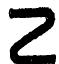
\includegraphics[keepaspectratio]{images/part001_40fd7be3.jpg}}

X 到 \(X'\) 上的等距映射当然是 X 的一致结构（相应地，拓扑）到 \(X'\) 的一致结构（相应地，拓扑）上的同构；这些命题的逆命题不成立，互不相同的等价度量的存在性（ \(\S\) 1，第 2 号）就表明了这一点。

设 X 是一个度量空间，d 是 X 上的度量。对每个 a \textgreater{} 0 ，用 \(V_{a}\) 表示 \(X \times X\) 的由所有点对 \((x, y)\) （满足 \(d(x, y) < a\) ）组成的子集，用 \(W_{a}\) 表示 \(X \times X\) 的由所有点对 \((x, y)\) （满足 \(d(x, y) \leqslant a\) ）组成的子集。当 a 取遍所有实数 \textgreater{} 0 组成的集（或仅仅取遍一个趋于 0 的 \textgreater{} 0 数列）时，诸集 \(V_{a}\) （相应地，\(W_{a}\) ）构成 X 的一致结构的开（相应地，闭）围域的一个基本系，这是由 d 的连续性得到的（§ 1，第 3 号）。我们有 \(\overline{V}_{a} \subset W_{a}\) ，但这两个集未必相同。

与 \(R^{n}\) 上欧氏距离的情形类比，集 \(\mathrm{V}_{a}(x)\) {[}相应地，\(\mathrm{W}_{a}(x)\) {]}称为以 x 为中心、以 a 为半径的开球（相应地，闭球）；它是 X 中的一个开（相应地，闭）集。又，由所有点 \(y \in X\) （满足 \(d(x, y) = a\) ）组成的集称为以 x 为中心、以 a 为半径的球面；它是一个闭集。由上所述，当 a 取遍所有实数 \textgreater0 组成的集或一个趋于 o 的 \textgreater0 数列时，以 x 为中心、以 a 为半径的开球（相应地，闭球）构成 x 的一个基本邻域系。

\pandocbounded{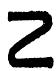
\includegraphics[keepaspectratio]{images/part001_d95d2d33.jpg}}

读者应当警惕，不要以为任意度量空间中的球与球面具有第六章，§ 2 中所研究的欧氏球与球面同样的性质。例如，开球的闭包未必是同一中心、同一半径的闭球；闭球的边界未必是同一中心、同一半径的球面；开球（或闭球）未必连通；而且球面可以是空集（参看习题 4）。

设 A 与 B 是度量空间 X 的任意两个非空子集。数

\[
d (\mathbf {A}, \mathbf {B}) = \inf _ {x \in \mathbf {A}, y \in \mathbf {B}} d (x, y)
\]

称为集合 A 与 B 之间的距离。特别地，我们用 \(d(x, \mathbf{A})\) 表示集合 \(\{x\}\) 与集合 A 之间的距离；它称为点 x 到集合 A 的距离。于是

\[
d (x, \mathrm{A}) = \inf _ {y \in \mathrm{A}} d (x, y)
\]

由此得

\[
d (\mathbf {A}, \mathbf {B}) = \inf _ {x \in \mathbf {A}} d (x, \mathbf {B})
\]

（第四章，§ 5，第 4 号，命题 9）。

注。若 \(d(x, \mathrm{A}) = a\) ，可能发生 A 中没有到 \(x\) 的距离等于 \(a\) 的点的情形。然而，若 A 是紧的，这种情形绝不会出现，因为这时魏尔斯特拉斯定理（第四章，§6，第 1 号，定理 1）表明，存在 \(y \in \mathrm{A}\) 使得 \(d(x, \mathrm{A}) = d(x, y)\) 。

命题 2. \(d(x, \mathbf{A}) = 0\) 与 \(x \in \overline{\mathbf{A}}\) 这两个陈述等价。

因为 \(d(x, \mathbf{A}) = 0\) 表明：球 \(\mathbf{V}_a(x)\) 与 \(\mathbf{A}\) 相交，无论 \(a > 0\) 取何值；而这等价于 \(x \in \overline{\mathbf{A}}\) 。

命题 3. 函数 \(d(x, \mathbf{A})\) 在 \(\mathbf{X}\) 上一致连续。

设 \(x\) 与 \(y\) 是 \(\mathbf{X}\) 中任意两点；则对任意给定的 \(\varepsilon > 0\) ，存在 \(z \in \mathbf{A}\) 使得 \(d(y, z) \leqslant d(y, \mathbf{A}) + \varepsilon\) ，因而

\[
d (x, z) \leqslant d (x, y) + d (y, z) \leqslant d (x, y) + d (y, A) + \varepsilon
\]

由三角不等式。

更有 \(d(x, \mathbf{A}) \leqslant d(x, y) + d(y, \mathbf{A}) + \varepsilon\) ，且由于 \(\varepsilon\) 是任意的，由此得 \(d(x, \mathbf{A}) \leqslant d(x, y) + d(y, \mathbf{A})\) 。类似地有

\[
d (y, \mathbf {A}) \leqslant d (x, y) + d (x, \mathbf {A}),
\]

从而

\[
\left| d (x, \mathbf {A}) - d (y, \mathbf {A}) \right| \leqslant d (x, y),\tag{2}
\]

由此即得结论。

注。可以有 \(d(\mathbf{A}, \mathbf{B}) = 0\) ，对某两个子集 \(\mathbf{A}, \mathbf{B}\) （\(\mathbf{X}\) 的子集）而言，它们满足 \(\overline{\mathbf{A}} \cap \overline{\mathbf{B}} = \emptyset\) ，只要这两个子集都不由单独一个点组成。例如，在实直线 \(\mathbf{R}\) 上，整数 \(> 0\) 组成的集与序列 \((n + 1/2n)_{n \geqslant 1}\) 的点组成的集是两个互不相交的闭集，它们之间的距离为零。

然而，若 A 紧且 B 闭，则关系 \(d(A, B) = 0\) 蕴含 \(A \cap B \neq \varnothing\) ，因为借助关系式

\[
d (\mathbf {A}, \mathbf {B}) = \inf _ {x \in \mathbf {A}} d (x, \mathbf {B})
\]

由命题 3 与魏尔斯特拉斯定理可知，存在 \(x_0 \in \mathbf{A}\) 使得 \(d(x_0, \mathbf{B}) = d(\mathbf{A}, \mathbf{B}) = 0\) ，从而（命题 2）\(x_0 \in \mathbf{B}\) 。

X 的非空子集 A 的直径是数（有限或等于 +∞）

\[
\delta (\mathbf {A}) = \sup _ {x \in \mathbf {A}, y \in \mathbf {A}} d (x, y).
\]

``W \(_{a}\) -小集''（第二章，§ 3，第 1 号）的概念与直径 \(\leqslant a\) 的集的概念相同。非空集 A 由单独一个点组成的必要充分条件是 \(\delta(\mathbf{A}) = 0\) 。

X 的子集 A （关于度量 d）称为有界的，如果它的直径有限；等价地，如果对每个点 \(x_{0} \in X\) ，A 都包含在以 \(x_{0}\) 为中心的一个球中。有界集的每个子集是有界的，且有限个有界集的并是有界集。

注意，X 的一个子集可以关于度量 d 有界，而关于与 d 等价的某个度量无界（参看 § 1，第 2 号）。

\subsection{函数的振幅}

与直径的概念相关的是函数 \(f\) （定义在任意集合 \(\mathbf{X}\) 上、取值于度量空间 \(\mathbf{X}'\) 中）的振幅的概念；若 \(\mathbf{A}\) 是 \(\mathbf{X}\) 的任意非空子集，则直径 \(\delta(f(\mathbf{A}))\) 称为 \(f\) 在 \(\mathbf{A}\) 中的振幅。

此外，若 \(\mathbf{X}\) 是拓扑空间 \(\mathbf{Y}\) 的子集，且 \(x \in \overline{\mathbf{X}}\) ，则数

\[
\omega (x; f) = \inf \delta (f (\mathbf {V} \cap \mathbf {X}))
\]

（当 V 取遍 \(x\) 在 Y 中的邻域滤子时）称为 \(f\) 在 \(x \in \overline{\mathbf{X}}\) 处的振幅。

命题 4. 振幅 \(\omega(x; f)\) ——任意函数 \(f\) （定义在拓扑空间 Y 的子集 X 上、取值于度量空间 \(\mathbf{X}'\) 中）的振幅—— 在 \(\overline{\mathbf{X}}\) 上是上半连续的。

设 \(a\) 是 \(\overline{\mathbf{X}}\) 中任意一点；则对每个 \(k > \omega(a; f)\) ，存在一个开邻域 \(\mathbf{V}\) （ \(a\) 的），使得 \(\delta(f(\mathbf{V} \cap \mathbf{X})) \leqslant k\) ；对每个 \(x \in \mathbf{V} \cap \overline{\mathbf{X}}\) ，\(\mathbf{V}\) 是 \(x\) 的一个邻域，因而

\[
\omega (x; f) \leqslant \delta (f (\mathbf {V} \cap \mathbf {X})) \leqslant k,
\]

这表明 \(\omega\) 在点 a 处上半连续。

为使 \(\omega(x; f) = 0\) 在点 \(x \in \overline{\mathbf{X}}\) 处成立，必要且充分的是：对每个 \(\varepsilon > 0\) ，存在一个邻域 \(\mathbf{V}\) （ \(x\) 的），使得 \(f(\mathbf{V} \cap \mathbf{X})\) 包含在半径为 \(\varepsilon\) 的一个球中；若 \(x \in \mathbf{X}\) ，这个条件表明 \(f\) 在点 \(x\) 处（关于 \(\mathbf{X}\) ）连续；若 \(x \in \overline{\mathbf{X}} \cap \complement \mathbf{X}\) ，则 \(f\) 映 \(\mathbf{X}\) 上的一个滤子基 —— \(x\) 在 \(\mathbf{Y}\) 中的邻域滤子的迹 —— 为 \(\mathbf{X}'\) 上的一个柯西滤子基；特别地：

命题 5. 设 \(f\) 是定义在一个子集 \(\mathbf{X}\) （拓扑空间 \(\mathbf{Y}\) 的子集）上、取值于完备度量空间 \(\mathbf{X}'\) 中的函数。则 \(f\) 关于 \(\mathbf{X}\) 在点 \(x \in \overline{\mathbf{X}}\) 处有极限的必要充分条件是 \(f\) 在 \(x\) 处的振幅为零。

\subsection{可度量化一致空间}

定义 2. 集合 X 上的度量称为与 X 上的一致结构 U 相容，如果由该度量定义的一致结构与 U 重合。

集合 X 上的一致结构称为可度量化的，如果存在 X 上的一个度量与这个一致结构相容。一致空间称为可度量化的，如果它的一致结构可度量化。

不同的度量可以与同一个一致结构相容；这时它们是等价的（§ 1，第 2 号，定义 2）。

定理 1. 一致结构可度量化的必要充分条件是：它是豪斯多夫的，且该一致结构的围域滤子具有可数基。

该条件是必要的，因为（用第 2 号的记号）围域 \(V_{1/n}\) （ \(n \geqslant 1\) ）构成度量空间的一致结构的围域滤子的一个基。

该条件是充分的，因为若该条件满足，则由第 1 节，第 4 号的命题 2，所考察的一致结构由单个伪度量定义；由于该一致结构是豪斯多夫的，这个伪度量是度量。

推论 1. 由可数族伪度量定义的豪斯多夫一致结构是可度量化的。

因为若 \((f_n)\) 是定义这样一个结构的伪度量序列，则围域滤子由集的可数族 \(\overline{f}_n^1([0, 1/m])\) 生成，其中 \(m\) 与 \(n\) 都取遍整数 \(>0\) 组成的集。

推论 2. 可度量化一致空间的每个可数乘积都是可度量化的。

因为这样的空间是豪斯多夫的，且它的一致结构具有可数的围域基本系（第二章，§ 2，第 6 号）。

\subsection{可度量化拓扑空间}

定义 3. 集合 X 上的度量称为与 X 上的拓扑 C 相容，如果由该度量定义的拓扑与 C 重合。拓扑空间称为可度量化的，如果存在 X 上的一个度量与 X 的拓扑相容。

\pandocbounded{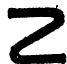
\includegraphics[keepaspectratio]{images/part001_d7e316f7.jpg}}

集合 X 上都与同一个拓扑 \(\mathfrak{C}\) 相容的两个度量可以不等价。

R 的子空间 \(R_{+}^{*}\) 提供了这样的一个例子。由 R 的加法一致结构诱导的一致结构与由 \(R^{*}\) 的乘法一致结构诱导的一致结构都是可度量化的，并且都与 \(R_{+}^{*}\) 的拓扑相容；但它们不可比较。

我们还指出，可以存在与可度量化拓扑空间的拓扑相容的不可度量化的一致结构（习题 7）。

这里我们只满足于给出拓扑空间可度量化的必要条件（关于必要充分条件，参看第 4 节，习题 22）。首先，一个空间除非是完全正则的，否则不可能是可度量化的（事实上我们将在第 4 节，第 1 号，命题 2 中看到，可度量化空间必然是``正规''的，这是一个更强的条件）。另一方面，定理 1 表明：

命题 6. 可度量化空间的每个点都具有可数的基本邻域系。

更一般地：

命题 7. 在可度量化空间中，每个闭集都是可数个开集之交，每个开集都是可数个闭集之并。

设 \(d\) 是与可度量化空间 \(\mathbf{X}\) 的拓扑相容的一个度量。若 \(\mathbf{A}\) 是 \(\mathbf{X}\) 的闭子集，则它是诸开集 \(\mathrm{V}_{1/n}(\mathbf{A})\) {[}由所有点 \(x\in\mathbf{X}\) （满足 \(d(x,\mathbf{A})<\mathbf{1}/n\) ）组成的集；参看命题 2{]}之交。命题的第二部分通过取余集得到。

注。1) 这些必要条件不是充分的（参看习题 13）。2) 存在这样的空间：其中每个点都有可数的基本邻域系，但其中存在不是可数个开集之交的闭集（习题 15）；这样的空间不是可度量化的。

第 4 节定理 1 的推论 2 表明，可度量化拓扑空间的可数乘积是可度量化的。此外，可度量化空间的任意族 \((\mathbf{X}_t)_{t \in \mathbf{I}}\) 的和 X （第一章，§ 2，第 4 号）也是可度量化的。因为若 \(d_t\) 是与 \(\mathbf{X}_t\) 的拓扑相容的度量（对每个 \(t \in \mathbf{I}\) ），则我们可以假定 \(d_t\) 有界且 \(\mathbf{X}_t\) 的直径 \(\leqslant t\) ；于是可以定义一个距离 \(d\) （与 \(\mathbf{X}\) 的拓扑相容）：规定 \(d(x, y) = d_t(x, y)\) 当 \(x\) 与 \(y\) 都属于同一个 \(\mathbf{X}_t\) 时，否则规定 \(d(x, y) = t\) 。

\subsection{可数序列的使用}

命题 6 是可度量化空间理论中点的可数序列所起作用的根源；对许多问题而言，可以用它们来有效地代替滤子。这是因为可度量化空间中点的邻域滤子（从而还有收敛滤子）由该空间中点的收敛序列确定：因为由于一点的邻域滤子具有可数基，它是比它细的诸基本滤子之交（第一章，§ 6，第 8 号，命题 11），即与收敛到所考察点的诸序列相伴随的基本滤子之交。

另一方面，收敛序列的概念不适用于研究这样的拓扑空间：其中有些点的邻域滤子没有可数基。特别地，可以构造非离散的豪斯多夫拓扑空间，使得在每个点 x 处，x 的邻域的任意可数族之交仍是 \(x (*)\) 的邻域；在这样的空间中，仅有的收敛序列是那些从某个指标起各项都相等的序列。

作为使用可数序列的例子，我们给出下列命题：

命题 8. 在可度量化空间 X 中，点 x 属于 X 的非空子集 A 的闭包，其必要充分条件是存在 A 的一个收敛到 x 的点列。

由第一章，§ 7，第 3 号我们已知该条件是充分的。为看出它是必要的，考察一个可数基本邻域系 \((\mathbf{V}_n)\) （ \(x\) 的），使得 \(\mathbf{V}_{n+1} \subset \mathbf{V}_n\) 对每个 \(n\) 成立。若 \(x\) 属于 A 的闭包，则每个 \(\mathbf{V}_n\) 与 A 相交，且若 \(x_n\) 属于 \(\mathbf{V}_n \cap \mathbf{A}\) ，则序列 \((x_n)\) 收敛到 \(x\) (**)。

由命题 8 我们推出：

命题 9. 度量空间 X 完备的必要充分条件是 X 中每个柯西序列都收敛。

设 \(\hat{\mathbf{X}}\) 是 \(\mathbf{X}\) 的完备化。若存在一点 \(x \in \hat{\mathbf{X}}\) 不属于 \(\mathbf{X}\) ，则存在一个序列 \((x_n)\) （\(\mathbf{X}\) 中的点的序列），它收敛到 \(x\) ，而这是 \(\mathbf{X}\) 中一个不收敛的柯西序列。

命题 10. 设 X 是可度量化空间，f 是 X 到拓扑空间 \(X'\) 中的一个映射。则 f 在点 \(x \in X\) 处连续的必要充分条件是：只要 \((x_n)\) 是 X 中收敛到 x 的点列，序列 \((f(x_n))\) 就收敛到 \(f(x)\) （在 \(X'\) 中）。

该条件是必要的，这由第一章，§ 7，第 4 号，命题 9 的推论 1 得到。为证明它是充分的，考察邻域滤子 \(\mathfrak{B}'\) —— \(f(a)\) 在 \(\mathbf{X}'\) 中的邻域滤子；假设蕴含 \(\overline{f}(\mathfrak{B}')\) 粗于与每个收敛到 \(a\) 的序列相伴随的基本滤子，也就是说粗于每个收敛到 \(a\) 的基本滤子；而这些滤子之交是 \(a\) 的邻域滤子（第一章，§ 6，第 8 号，命题 11）。由此即得结论。

注意，命题 8 与命题 10 在每个点都具有可数基本邻域系的任何空间 X 中都成立。

\subsection{可度量化空间上的半连续函数}

命题 11. 设 X 是可度量化空间，f 是 X 上取值于闭区间 \([a, b]\) （ \(\overline{R}\) 中的闭区间）的下半连续函数。则 f 是 X 上取值于 \([a, b]\) 中的连续函数组成的递增序列的上包络。

由结构转移，我们可以假定 \(a = 0\) 且 \(b = 1\) 。

\begin{enumerate}
\def\labelenumi{(\roman{enumi})}
\tightlist
\item
  先设 \(f = \varphi_{\mathbf{A}}\) ，其中 \(\mathbf{A}\) 是 \(\mathbf{X}\) 的一个开子集。则函数 \(g_n\) —— 由 \(g_n(x) = n\) . inf \((d(x, \mathbf{X} - \mathbf{A}), \mathfrak{r}/n)\) 定义 —— 连续且 \(\geqslant 0\) （在 \(\mathbf{X}\) 上）；而且 \(g_n(x) = f(x)\) 当 \(x \in \mathbf{X} - \mathbf{A}\) 以及当
\end{enumerate}

\[
d (x, \mathbf {X} - \mathbf {A}) \geqslant \mathrm{r} / n.
\]

时也成立。由此立即可得 \(f = \sup_{n}(g_n)\) 。

\begin{enumerate}
\def\labelenumi{(\roman{enumi})}
\setcounter{enumi}{1}
\tightlist
\item
  一般情形，对每个整数 \(n \geqslant 1\) ，考察开集的有限递减序列
\end{enumerate}

\[
\mathrm{A} _ {k} = \overline {{{f}}} ^ {1} \left(\right] \frac {k}{n}, + \infty [) \quad (0 \leqslant k \leqslant n - 1);
\]

函数 \(g_{n} = \frac{1}{n}\sum_{k=1}^{n-1}\varphi_{\mathbf{A}_k}\) 是下半连续的，且 \(0 \leqslant f(x) - g_{n}(x) \leqslant 1/n\) 对一切 \(n\) 成立；因而 \(f\) 是序列 \((g_n)\) 的上包络。另一方面，\(g_{n}\) 是有限多个开集的特征函数的具正系数的线性组合，因而它是可数序列 \((h_{mn})_{m \geqslant 0}\) （由连续函数 \(\geqslant 0\) 组成的序列）的上包络（由 (i)）；故 \(f = \sup_{m,n} h_{mn}\) 。若令 \(f_{n} = \sup_{p \leqslant n, q \leqslant n} h_{pq}\) ，则我们看到序列 \((f_n)\) 是连续函数 \(\geqslant 0\) 的一个递增序列，以 \(f\) 为上包络，且不取值 \(1\) ，因为 \(g_{n} \leqslant n - 1/n\) 。

\subsection{可数型可度量化空间}

定义 4. 可度量化空间称为可数型的（或可分的），如果它的拓扑具有可数基。

显然，可数型可度量化空间的每个子空间仍是可数型的。乘积空间拓扑基的定义（第一章，§ 4，第 1 号）与第 4 号定理 1 的推论 2 表明，可数个可数型可度量化空间的乘积是可数型可度量化空间。同样，可数个可数型可度量化空间的和是可数型可度量化空间（第 5 号）。

命题 12. 若 X 是可度量化拓扑空间，则下列陈述等价：

\begin{enumerate}
\def\labelenumi{\alph{enumi})}
\item
  X 是可数型的。
\item
  X 有可数稠密子集。
\item
  X 同胚于方体 IN 的一个子空间，其中 I 是 R 中的区间 {[}o, i{]} 。
\end{enumerate}

由前面的注记，显然 c) 蕴含 a)；a) 蕴含 b)，因为若 \((\mathbf{U}_{n})\) 是 X 的拓扑的一个可数基，且 \(a_{n}\) 是 \(U_{n}\) 的一个点，则诸 \(a_{n}\) 构成 X 的一个稠密子集。最后证明 b) 蕴含 c)。设 \((a_{n})\) 是 X 的点的稠密序列，且对每个 \(x \in X\) ，令 \(\varphi(x)\) 为点 \((d(x, a_{n}))_{n \in \mathbb{N}}\) —— \(I^{N}\) 的点 ——（d 是与 X 的拓扑相容、且关于它 X 的直径 \(\leqslant 1\) 的一个度量）。我们将证明 \(\varphi\) 是 X 到 \(I^{N}\) 的一个子空间上的同胚。事实上，\(\varphi\) 是连续的，因为每个函数 \(x \to d(x, a_{n})\) 都连续；且 \(\varphi\) 是单射，因为 X 的每个点都是 \((a_{n})\) 的某个子序列的极限（命题 8）。设 B 是 X 中以 \(x_{0}\) 为中心、以 r 为半径的一个球，并设 n 是使

\[
\left| d (x _ {0}, a _ {n}) <   \frac {1}{3} r. \right|
\]

\(\varphi\) 把集 \(W\) —— 由满足以下条件的点 \(x\in X\) 组成的集 ——

\[
\left| d (x _ {0}, a _ {n}) - d (x, a _ {n}) \right| <   \frac {1}{3} r
\]

映为按定义是 \(\varphi(x_0)\) 在 \(\varphi(\mathbf{X})\) 中的一个邻域。但对每个 \(x \in W\) 有 \(d(x, a_n) < d(x_0, a_n) + \frac{1}{3} r < \frac{2}{3} r\) ，由此得

\[
d (x, x _ {0}) \leqslant d (x _ {0}, a _ {n}) + d (x, a _ {n}) <   r,
\]

这表明 W 是包含在 B 中的 \(x_{0}\) 的一个邻域，因而 \(\varphi\) 是 X 到 \(\varphi(\mathbf{X})\) 上的一个同胚。

\pandocbounded{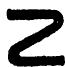
\includegraphics[keepaspectratio]{images/part001_a8399183.jpg}}

注意，对任意拓扑空间 X 而言，性质 b) 不一定蕴含可数基的存在性，即使 X 是紧的且 X 的每个点都有可数的基本邻域系（习题 13；参看第一章，§ 1，习题 7）。

命题 13. 设 X 是具有可数基 \((\mathbf{U}_n)\) 的拓扑空间；则对 X 的每个开覆盖 \((\mathbf{V}_t)_{i \in \mathbf{I}}\) ，存在 I 的可数子集 J，使得 \((\mathbf{V}_t)_{i \in \mathbf{J}}\) 是 X 的一个覆盖。

设 H 是由使 \(U_{n}\) 至少包含在某个 \(V_{t}\) 中的指标 n 组成的 N 的子集；序列 \((\mathrm{U}_{n})_{n\in\mathbf{H}}\) 是 X 的一个覆盖，因为每个点 \(x\in X\) 属于某个 \(V_{t}\) ，且由于 \(V_{t}\) 是开的，存在指标 n 使得 \(x\in U_{n}\subset V_{t}\) 。因而存在 H 到 I 中的一个映射 \(\psi\) ，使得 \(U_{n}\subset V_{\psi(n)}\) 对每个 \(n\in H\) 成立；取 \(J=\psi(H)\) ，它是可数的，命题得证。

\subsection{紧度量空间；紧可度量化空间}

一致空间预紧性的判别法（第二章，§ 4，第 2 号，定理 3）对度量空间给出下述命题：

命题 14. 度量空间 X 预紧的必要充分条件是：对每个 \(\varepsilon > 0\) ，存在 X 的由直径 \(\leqslant \varepsilon\) 的集组成的有限覆盖。

若再加上 X 完备这一假设，我们就得到度量空间紧性的一个判别法。

由命题 14 我们得到一个适用于可度量化空间的紧性拓扑判别法：

命题 15. 可度量化拓扑空间 X 紧的必要充分条件是：X 的每个无穷点列在 X 中有一个聚点。

第一章，§ 9，第 1 号的公理 (C) 表明该条件是必要的。为证明充分性，设 \(d\) 是与 \(\mathbf{X}\) 的拓扑相容的一个度量。我们先证明这样定义的度量空间 \(\mathbf{X}\) 是完备的：\(\mathbf{X}\) 中每个柯西序列都有聚点，从而是收敛的（第二章，§ 3，第 2 号，命题 5 的推论 2）；因而由命题 9，\(\mathbf{X}\) 是完备的。其次我们证明 \(\mathbf{X}\) 是预紧的；若非如此，则由命题 14，存在实数 \(\alpha > 0\) ，使得 \(\mathbf{X}\) 不能被 \(\mathbf{X}\) 的任何有限多个直径 \(\leqslant \alpha\) 的子集覆盖。于是我们可以对 \(n\) 用归纳法定义一个无穷序列 \((x_n)\) （\(\mathbf{X}\) 的点的序列），满足条件 \(d(x_p, x_n) > \frac{1}{2} \alpha\) 对一切 \(p < n\) 成立；而这样的序列不可能有聚点，因为每个半径 \(< \frac{1}{2} \alpha\) 的球至多包含该序列的一个点。

推论. 可度量化拓扑空间 X 的子集 A 相对紧的必要充分条件是：A 的每个无穷点列在 X 中有一个聚点。

设 \(d\) 是与 \(\mathbf{X}\) 的拓扑相容的一个度量。我们将应用命题 15 的判别法证明空间 \(\overline{\mathbf{A}}\) 是紧的。设 \((x_{n})\) 是 \(\overline{\mathbf{A}}\) 的点的一个序列；则对每个指标 \(n\) 存在 \(y_{n} \in \mathbf{A}\) 使得 \(d(x_{n}, y_{n}) < 1/n\) ；由假设，序列 \((y_{n})\) 有一个聚点 \(a \in \mathbf{X}\) ，且 \(a\) 也是序列 \((x_{n})\) 的聚点，因为若 \(y_{m}\) 位于以 \(a\) 为中心、以 \(1/n\) 为半径的球中（对某个 \(m > n\) ），则 \(x_{m}\) 位于以 \(a\) 为中心、以 \(2/n\) 为半径的球中。

应当指出，命题 15 并不是 X 的每个点处可数基本邻域系存在性的推论；存在不可度量化的、非紧的空间的例子，其中每个点都有可数的基本邻域系，且每个无穷点列都有聚点（习题 15）。

命题 16. 紧空间 X 可度量化的必要充分条件是它的拓扑具有可数基。

该条件是必要的。由命题 14，对每个整数 \(n \geqslant 1\) ，存在一个有限子集 \(A_n\) （\(X\) 的子集），使得 \(A_n\) 与 \(X\) 的每个点的距离 \(\leqslant 1/n\) ；因而可数集 \(A = \bigcup_{n} A_n\) 在 \(X\) 中稠密，于是由第 8 号的命题 12 即得结论。

该条件是充分的。设 \((\mathbf{U}_{n})\) 是 X 的拓扑的一个可数基。因而对角线 \(\Delta\) —— \(X \times X\) 的对角线 —— 的每个点的每个邻域都包含一个形如 \(U_{n} \times U_{n}\) 的邻域；对紧子集 \(\Delta\) （ \(X \times X\) 的紧子集）应用波莱尔–勒贝格公理可知，\(\Delta\) 的每个邻域都包含形如 \(U_{n} \times U_{n}\) 的集的一个有限并，而这样的并是 \(\Delta\) 的一个邻域。因而 \(\Delta\) 的这样的邻域——由形如 \(U_{n} \times U_{n}\) 的集的有限并组成的邻域——构成 X 的一致结构的一个围域基本系（第二章，§ 4，第 1 号，定理 1），于是由第 4 号的定理 1 即得结论。

推论. 设 X 是局部紧空间，X' 是通过给 X 添加一个无穷远点 ω 而得到的紧空间（第一章，§ 9，第 8 号）。则下列陈述等价：

\begin{enumerate}
\def\labelenumi{\alph{enumi})}
\item
  \(\mathbf{X}\) 的拓扑有可数基。
\item
  \(\mathbf{X}'\) 可度量化。
\item
  X 可度量化且是 \(\sigma\) -紧的。
\end{enumerate}

a) \(\Longrightarrow\) b)：设 \((\mathbf{U}_n)\) 是 \(\mathbf{X}\) 的拓扑的一个可数基。点 \(x \in \mathbf{X}\) 的每个邻域都包含 \(x\) 的一个紧邻域，而后者又包含 \(x\) 的一个等于某个 \(\mathbf{U}_n\) 的邻域。因而相对紧的诸 \(\mathbf{U}_n\) 构成 \(\mathbf{X}\) 的拓扑的一个基，于是我们可以假定所有 \(\mathbf{U}_n\) 都是相对紧的。因而 \(\mathbf{X}\) 是紧集 \(\overline{\mathbf{U}}_n\) 的可数并，即它是 \(\sigma\) -紧的；这蕴含在 \(\mathbf{X}'\) 中点 \(\omega\) 有由开邻域组成的可数基本系 \((\mathbf{V}_n)\) （第一章，§ 9，第 9 号，命题 15 的推论 2）。因而点 \(y \in \mathbf{X}'\) 的每个邻域都包含某个 \(\mathbf{U}_n\) 或某个 \(\mathbf{V}_n\) ，它是 \(y\) 的一个邻域，于是诸 \(U_{n}\) 与诸 \(V_{n}\) 构成 \(X'\) 的拓扑的一个可数基。因而由命题 16，\(X'\) 可度量化。

b) \(\Longrightarrow\) c): 若 \(X'\) 可度量化，则 \(\omega\) 有可数的基本邻域系，因而由第一章，§ 9，第 9 号，命题 15 的推论 2，\(X\) 是 \(\sigma\) -紧的。

c) \(\Longrightarrow a)\) ：由假设，存在相对紧开集的一个递增序列 \((\mathbf{V}_n)\) ，它们覆盖 \(\mathbf{X}\) 且满足 \(\overline{\mathbf{V}}_n \subset \mathbf{V}_{n+1}\) （第一章，§ 9，第 9 号，命题 15）。子空间 \(\overline{\mathbf{V}}_n\) 紧且可度量化，因而具有可数基（命题 16），从而 \(\mathbf{V}_n\) 也具有可数基。设 \((\mathbf{U}_{mn})_{m \geqslant 1}\) 是 \(\mathbf{V}_n\) 的拓扑的一个基。对每个 \(x \in \mathbf{X}\) 与每个邻域 \(W\) （ \(x\) 的），存在 \(n\) 使得 \(x \in \mathbf{V}_n\) ，因而存在 \(m\) 使得 \(x \in \mathbf{U}_{mn} \subset \mathbf{V}_n \cap W\) 。因而诸集 \(\mathbf{U}_{mn}\) （ \(m \geqslant 1\) ， \(n \geqslant 1\) ）构成 \(\mathbf{X}\) 的拓扑的一个基。
